% !TEX encoding = UTF-8 Unicode
% !TEX spellcheck = en_US
%  LaTeX support: latex@mdpi.com 
%  In case you need support, please attach all files that are necessary for compiling as well as the log file, and specify the details of your LaTeX setup (which operating system and LaTeX version / tools you are using).

%=================================================================
\documentclass[robotics,article,submit,moreauthors,pdftex]{Definitions/mdpi} 

% If you would like to post an early version of this manuscript as a preprint, you may use preprint as the journal and change 'submit' to 'accept'. The document class line would be, e.g., \documentclass[preprints,article,accept,moreauthors,pdftex]{mdpi}. This is especially recommended for submission to arXiv, where line numbers should be removed before posting. For preprints.org, the editorial staff will make this change immediately prior to posting.

%--------------------
% Class Options:
%--------------------
%----------
% journal
%----------
% Choose between the following MDPI journals:
% acoustics, actuators, addictions, admsci, aerospace, agriculture, agriengineering, agronomy, algorithms, animals, antibiotics, antibodies, antioxidants, applsci, arts, asc, asi, atmosphere, atoms, axioms, batteries, bdcc, behavsci , beverages, bioengineering, biology, biomedicines, biomimetics, biomolecules, biosensors, brainsci , buildings, cancers, carbon , catalysts, cells, ceramics, challenges, chemengineering, chemistry, chemosensors, children, cleantechnol, climate, clockssleep, cmd, coatings, colloids, computation, computers, condensedmatter, cosmetics, cryptography, crystals, dairy, data, dentistry, designs , diagnostics, diseases, diversity, drones, econometrics, economies, education, electrochem, electronics, energies, entropy, environments, epigenomes, est, fermentation, fibers, fire, fishes, fluids, foods, forecasting, forests, fractalfract, futureinternet, futurephys, galaxies, games, gastrointestdisord, gels, genealogy, genes, geohazards, geosciences, geriatrics, hazardousmatters, healthcare, heritage, highthroughput, horticulturae, humanities, hydrology, ijerph, ijfs, ijgi, ijms, ijtpp, informatics, information, infrastructures, inorganics, insects, instruments, inventions, iot, j, jcdd, jcm, jcp, jcs, jdb, jfb, jfmk, jimaging, jintelligence, jlpea, jmmp, jmse, jnt, jof, joitmc, jpm, jrfm, jsan, land, languages, laws, life, literature, logistics, lubricants, machines, magnetochemistry, make, marinedrugs, materials, mathematics, mca, medicina, medicines, medsci, membranes, metabolites, metals, microarrays, micromachines, microorganisms, minerals, modelling, molbank, molecules, mps, mti, nanomaterials, ncrna, neonatalscreening, neuroglia, nitrogen, notspecified, nutrients, ohbm, particles, pathogens, pharmaceuticals, pharmaceutics, pharmacy, philosophies, photonics, physics, plants, plasma, polymers, polysaccharides, preprints , proceedings, processes, proteomes, psych, publications, quantumrep, quaternary, qubs, reactions, recycling, religions, remotesensing, reports, resources, risks, robotics, safety, sci, scipharm, sensors, separations, sexes, signals, sinusitis, smartcities, sna, societies, socsci, soilsystems, sports, standards, stats, surfaces, surgeries, sustainability, symmetry, systems, technologies, test, toxics, toxins, tropicalmed, universe, urbansci, vaccines, vehicles, vetsci, vibration, viruses, vision, water, wem, wevj

%---------
% article
%---------
% The default type of manuscript is "article", but can be replaced by: 
% abstract, addendum, article, benchmark, book, bookreview, briefreport, casereport, changes, comment, commentary, communication, conceptpaper, conferenceproceedings, correction, conferencereport, expressionofconcern, extendedabstract, meetingreport, creative, datadescriptor, discussion, editorial, essay, erratum, hypothesis, interestingimages, letter, meetingreport, newbookreceived, obituary, opinion, projectreport, reply, retraction, review, perspective, protocol, shortnote, supfile, technicalnote, viewpoint
% supfile = supplementary materials

%----------
% submit
%----------
% The class option "submit" will be changed to "accept" by the Editorial Office when the paper is accepted. This will only make changes to the frontpage (e.g., the logo of the journal will get visible), the headings, and the copyright information. Also, line numbering will be removed. Journal info and pagination for accepted papers will also be assigned by the Editorial Office.

%------------------
% moreauthors
%------------------
% If there is only one author the class option oneauthor should be used. Otherwise use the class option moreauthors.

%---------
% pdftex
%---------
% The option pdftex is for use with pdfLaTeX. If eps figures are used, remove the option pdftex and use LaTeX and dvi2pdf.

%=================================================================
\firstpage{1} 
\makeatletter 
\setcounter{page}{\@firstpage} 
\makeatother
\pubvolume{xx}
\issuenum{1}
\articlenumber{5}
\pubyear{2019}
\copyrightyear{2019}
%\externaleditor{Academic Editor: name}
\history{Received: date; Accepted: date; Published: date}
%\updates{yes} % If there is an update available, un-comment this line

%% MDPI internal command: uncomment if new journal that already uses continuous page numbers 
%\continuouspages{yes}

%------------------------------------------------------------------
% The following line should be uncommented if the LaTeX file is uploaded to arXiv.org
%\pdfoutput=1

%=================================================================
% Add packages and commands here. The following packages are loaded in our class file: fontenc, calc, indentfirst, fancyhdr, graphicx, lastpage, ifthen, lineno, float, amsmath, setspace, enumitem, mathpazo, booktabs, titlesec, etoolbox, amsthm, hyphenat, natbib, hyperref, footmisc, geometry, caption, url, mdframed, tabto, soul, multirow, microtype, tikz
\graphicspath{{./figures/}}
\usepackage{calrsfs} % Für Kalligraphie-F 
\newcommand{\bm}[1]{\boldsymbol{#1}}
% Latex-Makros für häufig verwendete Formelzeichen
\DeclareMathOperator{\arctantwo}{arctan2}
\newcommand{\ortvek}[4]{{ }_{(#1)}{\boldsymbol{#2}}^{#3}_{#4} }
\newcommand{\vek}[3]{\boldsymbol{#1}^{#2}_{#3}}
\newcommand{\rotmat}[2]{{{ }^{#1}\boldsymbol{R}}_{#2}}
\newcommand{\rotmato}[2]{{{ }^{#1}\boldsymbol{\overline{R}}}_{#2}}
\newcommand{\transp}[0]{{\mathrm{T}}}
\newcommand{\ks}[1]{{\mathcal{F}}_{#1}}


%=================================================================
%% Please use the following mathematics environments: Theorem, Lemma, Corollary, Proposition, Characterization, Property, Problem, Example, ExamplesandDefinitions, Hypothesis, Remark, Definition
%% For proofs, please use the proof environment (the amsthm package is loaded by the MDPI class).

%=================================================================
% Full title of the paper (Capitalized)
\Title{Modeling Parallel Robot Kinematics for 3T2R and 3T3R Tasks using Reciprocal Sets of Euler Angles}

% Author Orchid ID: enter ID or remove command
%\newcommand{\orcidauthorA}{0000-0000-000-000X} % Add \orcidA{} behind the author's name
%\newcommand{\orcidauthorB}{0000-0000-000-000X} % Add \orcidB{} behind the author's name

% Authors, for the paper (add full first names)
\Author{Moritz Schappler $^{1,*}$, Svenja Tappe $^{1}$ and Tobias Ortmaier $^{1}$}

% Authors, for metadata in PDF
\AuthorNames{Moritz Schappler, Svenja Tappe and Tobias Ortmaier}

% Affiliations / Addresses (Add [1] after \address if there is only one affiliation.)
\address{%
$^{1}$ \quad Institut für Mechatronische Systeme, Leibniz Universität Hannover; firstname.lastname@imes.uni-hannover.de}

% Contact information of the corresponding author
\corres{Correspondence: moritz.schappler@imes.uni-hannover.de;}

% Current address and/or shared authorship
%\firstnote{Current address: Affiliation 3} 
%\secondnote{These authors contributed equally to this work.}
% The commands \thirdnote{} till \eighthnote{} are available for further notes

%\simplesumm{} % Simple summary

%\conference{} % An extended version of a conference paper

% Abstract (Do not insert blank lines, i.e. \\) 
\abstract{
Industrial manipulators and parallel robots are often used for tasks like drilling or milling, that require three translational, but only two rotational degrees of freedom (``3T2R'').
While kinematic models for specific mechanisms for these tasks exist, a general kinematic model for parallel robots is still missing.
This paper presents the definition of the rotational component of kinematic constraints equations for parallel robots based on two reciprocal sets of Euler angles for the end-effector orientation and the orientation residual.
The method allows to completely remove the redundant coordinate in 3T2R tasks and to solve the inverse kinematics for general serial and parallel robots with the gradient-descent algorithm.
The functional redundancy of robots with full mobility is exploited using nullspace projection.
%By exploiting functional redundancy of robots with full mobility in the nullspace of the gradient-descent algorithm, the mathematical complexity is low.
}
%A single paragraph of about 200 words maximum. For research articles, abstracts should give a pertinent overview of the work. We strongly encourage authors to use the following style of structured abstracts, but without headings: (1) Background: Place the question addressed in a broad context and highlight the purpose of the study; (2) Methods: Describe briefly the main methods or treatments applied; (3) Results: Summarize the article's main findings; and (4) Conclusion: Indicate the main conclusions or interpretations. The abstract should be an objective representation of the article, it must not contain results which are not presented and substantiated in the main text and should not exaggerate the main conclusions.}

% Keywords
\keyword{Parallel robot; five-DoF task; 3T2R task; functional redundancy; task redundancy; redundancy resolution; reciprocal Euler angles; inverse kinematics} % (list three to ten pertinent keywords specific to the article, yet reasonably common within the subject discipline.)

% The fields PACS, MSC, and JEL may be left empty or commented out if not applicable
%\PACS{J0101}
%\MSC{}
%\JEL{}

%%%%%%%%%%%%%%%%%%%%%%%%%%%%%%%%%%%%%%%%%%
% Only for the journal Diversity
%\LSID{\url{http://}}

%%%%%%%%%%%%%%%%%%%%%%%%%%%%%%%%%%%%%%%%%%
% Only for the journal Applied Sciences:
%\featuredapplication{Authors are encouraged to provide a concise description of the specific application or a potential application of the work. This section is not mandatory.}
%%%%%%%%%%%%%%%%%%%%%%%%%%%%%%%%%%%%%%%%%%

%%%%%%%%%%%%%%%%%%%%%%%%%%%%%%%%%%%%%%%%%%
% Only for the journal Data:
%\dataset{DOI number or link to the deposited data set in cases where the data set is published or set to be published separately. If the data set is submitted and will be published as a supplement to this paper in the journal Data, this field will be filled by the editors of the journal. In this case, please make sure to submit the data set as a supplement when entering your manuscript into our manuscript editorial system.}

%\datasetlicense{license under which the data set is made available (CC0, CC-BY, CC-BY-SA, CC-BY-NC, etc.)}

%%%%%%%%%%%%%%%%%%%%%%%%%%%%%%%%%%%%%%%%%%
% Only for the journal Toxins
%\keycontribution{The breakthroughs or highlights of the manuscript. Authors can write one or two sentences to describe the most important part of the paper.}

%\setcounter{secnumdepth}{4}
%%%%%%%%%%%%%%%%%%%%%%%%%%%%%%%%%%%%%%%%%%
\begin{document}
%%%%%%%%%%%%%%%%%%%%%%%%%%%%%%%%%%%%%%%%%%

%%%%%%%%%%%%%%%%%%%%%%%%%%%%%%%%%%%%%%%%%%
\section{Introduction}
\label{sec:intro}

%\color{gray}
%Einleitung ins Thema, Aufgabenredundanz, serielle Roboter
%\begin{itemize}
%	\item Parallele Roboter werden aufgrund ihrer hohen Steifigkeit in großem Ausmaß für Zerspanungsaufgaben verwendet, die mit 5 FG beschrieben werden können: 3T2R Task Space.
%	\item Dazu werden hauptsächlich Strukturen mit 6 EE-FG eingesetzt (3T3R Operational Space). Dadurch liegt eine Aufgabenredundanz vor, für deren gradientenbasierte Lösung es noch keine allgemeingültige Lösung für PKM gibt.
%	\item Für serielle Industrieroboter in 3T2R-Aufgaben gibt es bereits verschiedene allgemeingültige Verfahren zur Lösung der inversen Kinematik und der resultierenden Aufgabenredundanz \cite{Baron2000,HuoBar2005,Zlajpah2017,LegerAng2016,ZhuQuCaoYan2013,GuoDonKe2015,MousaviGagBouRay2018,1_SchapplerTapOrt2019}
%	\item Die gradientenbasierten Verfahren \cite{Baron2000,HuoBar2005,Zlajpah2017,LegerAng2016,1_SchapplerTapOrt2019} ermöglichen die Projektion zusätzlicher Optimierungskriterien in den Nullraum des Gradienten und somit auch die Ausnutzung der Aufgabenredundanz durch gleichzeitige Optimierung der Nebenbedingungen mit der Lösung des IK-Problems.
%	\item Die Bildung eines an 3T2R-Aufgaben angepassten Residuumsvektors und des dazu passenden Gradienten erfolgt dabei auf unterschiedliche Weise, wie bspw. Hinzufügen einer virtuellen Achse \cite{Baron2000}, Zerlegung des Task Space \cite{HuoBar2005}, Rotation in Task Frame und weglassen einer Komponente \cite{Zlajpah2017}, Definition der Werkzeugachse durch zwei Punkte und daraus Konstruktion eines Nullraums \cite{LegerAng2016}, Definition von absoluter Orientierung und Orientierungsfehler mit reziproken Euler-Winkeln \cite{1_SchapplerTapOrt2019}.
%\end{itemize}
%\color{black}

Industrial tasks like welding, gluing, milling or drilling represent a major part the of applications of industrial robots, which generally have full mobility, i.\,e. the operational space of their end-effector has three translational and three rotational (``3T3R'') degrees of freedom (``DoF'').
Parallel robots like the Stewart-platform have especially been proposed for milling tasks regarding their high structural stiffness.
The task space of the named applications can be defined by three translational DoF and only two rotations due to a symmetry around the tool axis (``3T2R'').
This results in a functional or task redundancy, which is not exploited to full extend yet for \emph{parallel} robots.

\subsection{Inverse Kinematics and Resolution of Task Redundancy for Serial Robots}

Various general gradient-based methods exist to solve the inverse kinematics for \emph{serial} robots; either by augmenting the joint space \cite{Baron2000} or by reducing the task space \cite{HuoBar2005,LegerAng2016,Zlajpah2017,1_SchapplerTapOrt2019}.
The different approaches each define a residual vector and a gradient matrix considering the properties of 3T2R tasks, e.\,g. by adding a virtual joint axis \cite{Baron2000}, orthogonal decomposition of the task space \cite{HuoBar2005}, rotation of the residual into a task frame and removing the corresponding component \cite{Zlajpah2017}, defining the tool axis by two points for constructing a nullspace \cite{LegerAng2016} or by defining the absolute orientation and the orientation residual with two reciprocal sets of Euler angles \cite{1_SchapplerTapOrt2019}.
The gradient matrices corresponding to the different residuals are used for an iterative Newton-Raphson algorithm \cite{Yoshikawa1984,GoldenbergBenFen1985} by exploiting the functional redundancy with a null space projection of additional performance criteria \cite{Yoshikawa1984}.
Without the definition of a proper gradient, a global optimization has to be performed outside of the inverse kinematics algorithm \cite{ZhuQuCaoYan2013,GuoDonKe2015}.

%\color{gray}
%Beschreibung des aktuellen Stands von PKM für 3T2R.
%\begin{itemize}
%	\item Für den Einsatz von PKM in 3T2R-Aufgaben gibt es unterschiedliche Ansätze \cite{Tale-MasoulehGos2011}: Asymmetrische 5FG (1), Symmetrische 5FG (2), 6FG-Mechanismen, die als 5FG redundant geregelt werden (3).
%	\item Die Nutzung einer aktiven Beinkette mit 3T2R-FG oder einer passiven Führungsstrebe mit 3T2R-FG setzt bei der Mobilität an. Dadurch hat die Plattform auch 3T2R-FG.
%	\item Dieses Konzept wird in der Literatur an verschiedenen Maschinentypen gezeigt:
%	\cite{WangGos1997} für 5UPS/US, \cite{ZhangGos2001} für 5UPS/RUU, \cite{LiuXuYaoXu2015,WenQinZhaLam2016} für 6PUS/UPU, \cite{ZhengGaoZha2005,GaoSunZha2004} für 5UPS/PRPU, \cite{Gogu2006} mit Isoglide5-A1 (3PRRRRR-2PRRRR), \cite{SchreiberGos2003} mit 4URS-1URU, \cite{MbarekNefCor2005,LinLiYanZha2013} mit 4UPS-1UPU oder \cite{GaoPenZhaLi2006} mit 4PSU-1PU*U. Durch die kinematische Struktur hat der EE immer nur 3T2R FG und eine Aufgabenredundanz liegt nicht vor. Die 5UPS-PRPU Maschine aus \cite{ChengWanZha2008} weist zusätzlich eine Antriebsredundanz auf.
%	\item In \cite{HuangLi2002} wurde mit Hilfe der Schraubentheorie am Bsp der 5UPU gezeigt, dass die Maschine nur lokale, und keine globale Mobilität aufweist, wenn die 5FG der Beinketten nicht übereinstimmen. Am Beispiel der Metrom-Maschine \cite{BaerWei2006}, der dazu ähnlichen 4SPRR-1PSPR-Maschine von \cite{AlaghebandMahMilBen2015} oder der Isoglide5 \cite{Gogu2006} wird deutlich, dass bei mehreren Beinketten mit 5FG der nicht durch die Aufgabe vorgegebene Rotations-FG um die Werkzeugachse bei allen Beinketten vorliegen muss. Das führt zu einer letzten Drehachse jeder Beinkette in der Werkzeugachse. Bei der konstruktiven Umsetzung wird das letzte Gelenk als rotierender Ring um die Werkzeugachse gewählt \cite{BaerWei2006,AlaghebandMahMilBen2015}.
%	\item Davon abweichend werden in \cite{KongGos2005} 5FG-PKM synthetisiert, die symmetrische Beinketten aufweisen. Diese werden in \cite{Tale-MasoulehGos2011} für 5RPUR und in \cite{Tale-MasoulehSaaGosTag2010} für 5PRUR genauer analysiert.
%	\item Bei Maschinen mit 3T3R EE-FG wie der Eclipse-Maschine (3PPRS) \cite{HongKim2000} oder Hexapod-Maschinen mit 6UPS-Struktur \cite{MerletPerDan2000}, die für 3T2R eingesetzt werden, kann der Drehwinkel des Endeffektors um die Symmetrieachse des Werkzeugs frei gewählt werden.
%\end{itemize}
%\color{black}

\subsection{Overview of Parallel Robots Structures for 3T2R tasks}
\label{sec:parrob_classification}

Parallel robots in 3T2R tasks can be ordered in classes according to their kinematic structure into
\begin{itemize}
	\item[I] mechanisms with full platform mobility (3T3R) that are redundantly controlled to five DoF,
	\item[II] mechanisms with 3T2R platform mobility enforced with a passive five-DoF constraining leg and five other legs with six DoF each,
	\item[III] mechanisms with 3T2R platform mobility resulting from the mobility of five actuated legs with five or six DoF each,
	\item[IV] mechanisms with 3T2R platform mobility and five legs with only five DoF each.
\end{itemize}

The classes I and II were introduced in \cite{Tale-MasoulehGos2011}, where class IV is analyzed regarding leg symmetry and singularities.
Class III is mainly influenced by the systematic synthesis of \cite{Gogu2008} and several existing prototypes and is demarcated against class II by the absence of the passive constraining leg.
Class IV can be seen as a subclass of III, but is differentiated in this paper due to its characteristics.
Other classifications are provided e.\,g. by \cite{HuangLiuChe2011}, where IV and II are termed ``families''.

Examples for the first class are hexapods\footnote{The joint structure is denoted by the number of the legs and the order of universal (``U''), prismatic (``P''), spherical (``S''), helical (``H'') and revolute (``R'') joints in the leg chains. Different actuated legs are connected by dashes (``-''), passive constraint legs are connected by a slash (``/''). Actuated joints are underlined.} (6U\underline{P}S) \cite{MerletPerDan2000} or the Eclipse \cite{HongKim2000} machine tool (2\underline{PPR}S-\underline{PP}RS).
Any other parallel robot with full mobility (see e.\,g. \cite{Merlet2006,Gogu2008,Zhang2009}) may be used as well.

The second class allows for more variety, since the six-DoF mechanism and the five-DoF constraining leg can manifest in different kinematic structures:
The U\underline{P}S structure is used for the six-DoF part of the mechanism 
  by \cite{WangGos1997} with a focus on kinematic analysis of 5U\underline{P}S/US, 
  by \cite{ZhangGos2001} with a focus on kinetostatic modeling at the example of 5U\underline{P}S/RUU (see Fig.\,\ref{fig:systems_pictures}\,a), 
  by \cite{ZhengGaoZha2005} with focus on trajectory control of 5U\underline{P}S/PRPU and 
  by \cite{GaoSunZha2004} for pose measurement with the passive leg of 5U\underline{P}S/PRPU.
Other possible general base structures are \underline{R}US at the 5\underline{R}US/US example in \cite{WangGos1997}, \underline{P}US, which has been investigated for the control of a redundantly actuated 6\underline{P}US/UPU regarding the control of the redundant leg with inverse-dynamics control \cite{LiuXuYaoXu2015} or force control \cite{WenQinZhaLam2016}.
%The redundantly actuated 5U\underline{P}S-\underline{P}RPU from \cite{ChengWanZha2008} is based on the machine from \cite{ZhengGaoZha2005}, but does not fall in any of the classes I-IV.

The most-straightforward member of the third class is the 4U\underline{P}S-U\underline{P}U of Fig.\,\ref{fig:systems_pictures}\,b, which is investigated in \cite{MbarekNefCor2005} for a simulation and feasibility study together with a survey on possible architectures for a technical realization of this class.
Other possible structures are 
  the 4U\underline{R}S-U\underline{R}U, which is analyzed kinematically in \cite{SchreiberGos2003} and
  the 4\underline{P}SU-\underline{P}U*U, which has a special parallelogram structure in one leg (termed ``U*'') and is presented in \cite{GaoPenZhaLi2006}.
A sub-class of III consists of mechanisms \cite{BaerWei2006,LinLiYanZha2013,AlaghebandMahMilBen2015}, where the last joint axis of the legs is coaxial with the tool axis and is constructed as rotating ring.
It contains the
  Metrom machine tool (4S\underline{P}RR-S\underline{P}R), depicted in Fig.\,\ref{fig:systems_pictures}\,c, which is analyzed regarding inverse and forward kinematics in \cite{BaerWei2006} or its variants, 
  the redundant 4S\underline{P}RR-\underline{P}S\underline{P}R from \cite{AlaghebandMahMilBen2015} or 
  the hybrid 4UR\underline{H}U-UR\underline{H}R with an additional linear actuator at the platform \cite{LinLiYanZha2013}.
%The last joint axis of the legs of this sub-class \cite{BaerWei2006,LinLiYanZha2013,AlaghebandMahMilBen2015} is coaxial with the tool axis and is constructed as rotating ring.
A structural synthesis based on linear transformations and evolutionary morphology \cite{Gogu2008} led e.\,g. to the Isoglide5 mechanisms (3\underline{P}RRRRR-2\underline{P}RRRR), which are analyzed and optimized regarding the isotropy of the Jacobian in \cite{Gogu2006}.

The simplest member of class IV, the 5U\underline{P}U is shown in \cite{HuangLi2002} with the help of screw theory to only have local mobility and no global mobility, since the twist systems of the leg chains have no intersection and the resulting twist system of the platform is empty.
Members of class IV have been found by systematic structural synthesis with screw theory, which has been performed in \cite{KongGos2005} for symmetric 3T2R mechanisms.
The resulting 5R\underline{P}UR of Fig.\,\ref{fig:systems_pictures}\,d and 5\underline{P}RUR are analyzed in \cite{Tale-MasoulehGos2011,Tale-MasoulehSaaGosTag2010}.
%
\begin{figure}[h!]
	\input{./figures/systems_pictures.pdf_tex}
	\caption{Typical mechanisms of the different classes. Taken from \cite{ZhangGos2001} (a), \cite{MbarekNefCor2005} (b), \cite{AlaghebandMahMilBen2015} (c), \cite{Tale-MasoulehGos2011} (d).}
	\label{fig:systems_pictures}
	\vspace{-0.4cm}	% Damit Fußnote von unten näher an das Bild heranrückt
\end{figure} 
\newpage
%
In a practical application with competing requirements on workspace, stiffness, costs and precision, each of the existing systems has its legitimization.
Nevertheless, each of the classes has inherent disadvantages:
In tasks like milling with high process forces and requirements on stiffness and precision, robots from class II with one constraining leg have the drawback, that the passive leg takes the complete reaction wrench in the blocked rotational degree of freedom, which strongly affects the mechanisms stiffness in this direction \cite{ZhangGos2001}.
The same is argued by \cite{LinLiYanZha2013} at the example of the Metrom machine tool, but can be extended to all the members of class III, where most leg chains have six DoF and usually only one leg chain has five DoF.
This leg chain also has to take the reaction moments in the blocked DoF which affects the overall stiffness.
Therefore members of the classes I and IV can be expected to reach a higher stiffness.
Mechanisms of the class IV may further suffer from an increased sensitivity of manufacturing tolerances, which may cause a high pretension of the bearings or even reduce the DoF, since the five DoF of all leg chains have to coincide exactly to allow the platform to also have five DoF.
Additionally, only members of class I provide redundancy which allows to use the additional DoF for performance optimizations e.\,g. to avoid singularities and to compensate the smaller workspace caused by the sixth leg.

Therefore, the remainder of the paper focuses on mechanisms of the first class to allow an optimization of their performance criteria using the degree of task redundancy.

%\color{gray}
%Methoden zur Lösung der IK. Methoden durchnummerieren und Tabelle mit allen Systemen machen. Dann verschiedene Paper und Roboter den nummerierten Methoden zuordnen.
%\begin{itemize}
%	\item Für die vorgestellten Maschinen mit 5 EE-FG \cite{LiuXuYaoXu2015,WenQinZhaLam2016,ZhengGaoZha2005,GaoSunZha2004,ChengWanZha2008,AlaghebandMahMilBen2015,BaerWei2006,Tale-MasoulehSaaGosTag2010,Tale-MasoulehGos2011} ist die inverse Kinematik analytisch einfach zu erhalten. Die Berechnung erfolgt durch die Definition der EE-Orientierung mit zwei mitgedrehten Winkeln für die Führungskette, die 3T2R-FG aufweist. Für die restlichen Ketten wird die IK dann analytisch mit Standard-Verfahren berechnet, da die Beinketten eine einfache Struktur aufweisen.
%	\item In \cite{MerletPerDan2000} wird die IK für eine 3T3R PKM (6UPS) in Abhängigkeit des Drehwinkels um die Werkzeugachse bestimmt. Der Drehwinkel wird dann mit einer Optimierung und Intervallanalyse gewählt. Mit dem Verfahren ist allerdings keine gradientenbasierte Optimierung der Nebenbedingungen möglich. Da hierbei ähnlich wie in \cite{ZhuQuCaoYan2013,GuoDonKe2015} für serielle Roboter kein Gradient definiert wird, muss eine aufwändigere globale Optimierung durchgeführt werden, bei der der redundante Winkel als Parameter variiert wird.
%\end{itemize}
%\color{black}

\subsection{Inverse Kinematics of Parallel Robots for 3T2R Tasks}

The parallel robots with five DoF presented previously have a kinematic structure, that allows for an analytic model of the inverse kinematics.
All references define the end-effector orientation with two consecutive elementary rotations, i.\,e. define two Euler angles to represent the tool axis orientation in minimal coordinates \cite{LiuXuYaoXu2015, WenQinZhaLam2016, ZhengGaoZha2005,GaoSunZha2004, ChengWanZha2008, AlaghebandMahMilBen2015, Tale-MasoulehSaaGosTag2010, BaerWei2006, Tale-MasoulehGos2011}, which is called ``partial pose'' in \cite{MerletPerDan2000}.
The inverse kinematics problem (IKP) is first solved for the first chain, which is called ``leading chain'' in this paper.
Due to the geometry of the leading chain, this solution can be found algebraically. %  \cite{WangGos1997}
Then the IKP is solved for the other ``following'' chains with the given orientation from the leading chain and standard methods.
For robots of class II, the constraining leg is selected as the leading leg chain and for class III the 3T2R leg is selected. %  \cite{WangGos1997}

To the best knowledge of the authors, only one reference \cite{MerletPerDan2000} for the IKP of functionally redundant parallel robots of the class I is known.
The reason presumably is that a solution of the 3T3R IKP for these robots is possible with standard methods, as used in \cite{HongKim2000} for the 3T3R Eclipse.
It is always possible to transfer the 3T2R IKP into 3T3R by adding an arbitrary value for the desired rotation around the tool axis.
An optimization of additional performance criteria is possible by varying the redundant rotation angle \cite{ZhuQuCaoYan2013,GuoDonKe2015}.
This approach was chosen in \cite{MerletPerDan2000} by first defining the IKP with the redundant rotation as a parameter and then performing an optimization of this parameter using analytical computation of the dexterity and interval analysis to ensure a minimum determinant of the inverse Jacobian.
The drawback of this method is the need for a cascaded optimization which is more complex than a gradient-based approach presented in this paper.

%\color{gray}
%Problembeschreibung, Ansatz des Papers
%\begin{itemize}
%	\item Die Übersicht zeigt, dass bisher keine allgemeinen Ansätze zur Redundanzauflösung von PKM für 3T2R-Aufgaben bekannt sind.
%	\item Die Arbeiten konzentrieren sich entweder auf eine allgemeine Struktursynthese dieser Maschinenstruktur basierend z.B. auf Schraubentheorie \cite{KongGos2005} oder der Theorie der linearen Transformation \cite{Gogu2006}. Für die Auswahl der Maschine für eine gegebene Aufgabe ist allerdings nicht nur die kinematische Struktursynthese, sondern auch die Maßsynthese entscheidend. Diese kombinierte Struktur- und Maßsynthese folgt dem Schema aus Bild \ref{fig:structdimsynth} und benötigt auch eine allgemeingültige Berechnung der IK, was aufgrund der Vielzahl der Systeme mit manuellen, analytischen Verfahren nicht umsetzbar ist.
%\end{itemize}
%\color{black}

\subsection{Motivation and Summary of the State of the Art}

The overview over the literature shows, that no general, machine-independent methods for the resolution of functional redundancy for 3T3R PKM in 3T2R tasks exists.
The works either focus on a general structural synthesis of machines e.\,g. via screw theory \cite{KongGos2005} or linear transformations \cite{Gogu2006} or the description and improvement of specific, manually selected, machines.
To choose the best machine for given requirements, a structural synthesis is only the first step.
Additionally, a dimensional synthesis should be performed for all possible structures to select the most suitable mechanism.
This combined structural and dimensional synthesis \cite{RamirezKotOrt2015} is sketched in Fig.\,\ref{fig:structdimsynth}.
To be able to perform the dimensional synthesis for all structures, the inverse kinematics has to be implemented in a general form, to calculate the performance criteria over a given trajectory for further optimization of the structures and their comparison.
For the generation of task redundant parallel robots, the inverse kinematics has to include an optimization of the performance criteria and the restrictions such as joint limits, to ensure a comparability of the results.
%
\begin{figure}[tb]
	\input{./figures/comb_struct_dim_synth.pdf_tex}
	\caption{Overview of the procedure for combined structural and dimensional synthesis.}
	\label{fig:structdimsynth}
\end{figure} 
%
%\color{gray}
%Beitrag des Papers:
%\begin{itemize}
%	\item Aufbauend auf der Beschreibung der Kinematik mit reziproken Euler-Winkeln \cite{1_SchapplerTapOrt2019} wird ein allgemeines, gradientenbasiertes Verfahren für die IK von PKM vorgestellt
%	\item Damit ist es möglich, sowohl PKM mit strukturell 3T2R-FG und Aufgabenredundante PKM mit 3T3R-PKM zu berücksichtigen.
%	\item Durch das gradientenbasierte Verfahren, in dem die redundante task space Koordinate komplett eliminiert wird, ist eine effiziente Umsetzung gegeben, die in der Bahnplanung und für Nullraum-Bewegungen der Maschinen eingesetzt werden kann.
%\end{itemize}
%\color{black}
%
To address this, the contributions of this paper are
\begin{itemize}
\item a general kinematics model for parallel robots using the concept of reciprocal Euler angles \cite{1_SchapplerTapOrt2019},
\item a complete elimination of the redundant operational space coordinate in this formulation for 3T2R tasks allowing a nullspace optimization in the gradient-based inverse kinematics,
\item proofs, examples and simulations to show the performance for single serial kinematic leg chains and complete parallel robots.
\end{itemize}

%\color{gray}
%Rest ist gegliedert:
%\begin{itemize}
%    \item Problembeschreibung: Inverse Kinematik von PKM bzw. Kinematik-Modellierung Kap \ref{sec:PKM_general}
%	\item Vorstellung des REW-Verfahrens aus \cite{1_SchapplerTapOrt2019} zur Modellierung serieller kinematischer Ketten Kap \ref{sec:REW_seriell}
%	\item Aufstellung der vollständigen kinematischen Zwangsbedingungen für allgemeine PKM mit dem Verfahren, Kap. \ref{sec:ZB_PKM}
%	\item Lösung des IK-Problems mit Redundanzauflösung und weitere Anwendungen der Modellierung Kap. \ref{sec:ZB_Anwendung}
%	\item Darstellung der Ergebnisse an Beispielsystemen, Kap. \ref{sec:Ergebnisse}
%\end{itemize}
%\color{black}

The remainder of the paper is structured as follows:
The description of the inverse kinematics problem and prior definitions are given in Sec.\,\ref{sec:PKM_general} and the concept of reciprocal Euler angles from \cite{1_SchapplerTapOrt2019} is adapted in Sec.\,\ref{sec:REW_seriell} for parallel robots.
This leads to the full kinematic constraints of parallel robots in 3T2R tasks, introduced in Sec.\,\ref{sec:ZB_PKM} and applied to the differential kinematics in Sec.\,\ref{sec:ZB_Anwendung}.
The theoretical analysis is followed by examples and simulations in Sec.\,\ref{sec:Ergebnisse}.
The appendix contains proofs and additional details on the mathematical formulation.

%%%%%%%%%%%%%%%%%%%%%%%%%%%%%%%%%%%%%%%%%%
\section{Inverse Kinematics Problem for Parallel Robots}
\label{sec:PKM_general}

%\color{gray}
%\begin{itemize}
%    \item Beschreibung des Systems und der Nomenklatur mit Bild (3RRR und 3RPR, eingezeichnete Vektoren)
%    \item Darstellung der kinematischen Zwangsbedingungen als Vektoren und für Betrag der Beinlänge. Vektor rAB und r0E einzeichnen
%    \item Eigenschaft nennen: Methode nicht allgemein, sondern Voraussetzung, dass nur die ersten Gelenkwinkel die Zwangsbedingungen beeinflussen
%    \item Hinweis Dynamik-Modellierung basiert auch auf diesen Zwangsbedingungen \cite{Merlet2006,BriotKha2015,AbdellatifHei2009,DoThanhKotHeiOrt2009b} und funktioniert auch nur für Roboter, mit diesen Eigenschaften
%    \item \cite{Gogu2008} nimmt allgemeine lineare Transformation für Position und Orientierung, aber auf Geschwindigkeitsebene. Damit die inverse Kinematik nicht direkt lösbar und nur für 3T3R.
%    \item Formeln: Kinematik der Beinkette und der Plattform, Kinematische Zwangsbedingungen in allgemeiner Form, Einfluss der Beingelenke anhand der Einträge in der Gradientenmatrix
%    \item Einschränkung schreiben: Methode nicht für allgemeine PKM anwendbar, die automatisch generiert werden, da immer analytisch die Systeme speziell gelöst werden
%    \item Skizzierung des Problems für 3T2R: Unterschiedliche Modellierung für Führungskette und Folgekette, Führungskette in Kap. \ref{sec:REW_seriell}, Folgekette und Zusammenschluss in Kap. \ref{sec:ZB_PKM}.
%    \item Bis hier noch keine rotatorischen Zwangsbedingungen hinschreiben. Die kommen erst in den folgenden Kapiteln
%\end{itemize}
%\color{black}

%\begin{figure}[tb]
%    \input{./figures/pkm_constr_def_transl.pdf_tex}
%    \caption{Kinematic Description of Parallel Robots.}
%    \label{fig:pkm_constr_transl}
%\end{figure} 

Before addressing the specific model for parallel robots in 3T2R tasks in the next section, the standard kinematics model of kinematics of parallel kinematic machines (``PKM'') is repeated in the following, corresponding to the state of the art \cite{Merlet2006,Gogu2008,BriotKha2015} and serving as a reference to highlight its shortcomings for 3T2R tasks.
The regarded parallel robot consists of $m$ legs, which each have the joint coordinates $\bm{q}_i$.
All joints are considered as single-DoF and additionally to the active joints $\bm{q}_{i,\mathrm{a}}$ explicitly all passive joints at the base and at the platform $\bm{q}_{i,\mathrm{p}}$ are included in the coordinates $\bm{q}_i$ of leg~$i$.
The coordinates
%
\begin{equation}
\bm{x}
=
\begin{bmatrix}
\bm{x}_{\mathrm{t}}^\transp & \bm{x}_{\mathrm{r}}^\transp
\end{bmatrix}^\transp
\in {\mathbb{R}}^{6}
\label{equ:x_def}
\end{equation}
%
of the end-effector platform describe the position and orientation of the end-effector frame  $\ks{D}$ with respect to the base frame $\ks{0}$.
In the equations, this is marked with left subscript ``$(0)$'' for vectors and left superscript ``$0$'' for rotation matrices.
The platform-related end-effector frame is the desired frame in the inverse kinematics problem and is therefore abbreviated with ``D''.
The position 
%
\begin{equation}
\bm{x}_{\mathrm{t}}
=
\ortvek{0}{r}{}{D}
\in {\mathbb{R}}^{3}
\label{equ:xt_def}
\end{equation}  
%
is defined as the origin of the platform frame and the rotation matrix
%
\begin{equation}
\rotmat{0}{D} (\bm{x}_{\mathrm{r}})
=
\begin{bmatrix}\vek{n}{}{D} & \vek{o}{}{D} & \vek{a}{}{D}\end{bmatrix} \in \mathrm{SO(3)}
\label{equ:xr_def_rotmat}
\end{equation}
%
of the platform frame is expressed with Euler angles
%
\begin{equation}
\bm{x}_{\mathrm{r}}
=
\begin{bmatrix}
\beta_1  & \beta_2 & \beta_3
\end{bmatrix}^{\mathrm{T}}
=:
\bm{\beta}
\in {\mathbb{R}}^{3}
\label{equ:xr_def}
\end{equation} 
%
as a minimal representation of the orientation coordinates.
The symbol ``$\bm{\beta}$'' will be used to denote orientations relative to the base frame throughout this paper.
The $X$-$Y$-$Z$-notation
%
\begin{equation}
\bm{R}(\bm{\beta}) = \bm{R}_x(\beta_1) \bm{R}_y(\beta_2) \bm{R}_z(\beta_3) \in \mathrm{SO(3)}
\label{equ:def_rmat_xyz}
\end{equation}
%
is used for the Euler angles without loss of generality.
%
The relation between joint coordinates $\bm{q}$ and platform coordinates $\bm{x}$ is established with the kinematic constraint equations, for which most commonly the vector loop
%
\begin{equation}
\bm{\Phi}_{\mathrm{t},i}(\bm{q}_i,\bm{x}) = - \ortvek{0}{r}{}{A_iB_i}(\bm{x}) + \ortvek{0}{r}{}{A_iB_i}(\bm{q}_i) 
\label{equ:kinconstrAB}
\end{equation}
%
between the position of the platform coupling point $B_i$ relative to the base coupling point $A_i$ is used for each leg chain $i$ \cite{Merlet2006}.
The second term $\ortvek{0}{r}{}{A_iB_i}(\bm{q}_i)$ corresponds to the forward kinematics of the serial leg chain. 
The vector
\begin{equation}
\ortvek{0}{r}{}{A_iB_i}(\bm{x}) = 
- \ortvek{0}{r}{}{A_i}
+ \bm{x}_{\mathrm{t}} + \rotmat{0}{D}(\bm{x}_{\mathrm{r}}) \ortvek{D}{r}{}{B_i}
\label{equ:vec_AB}
\end{equation}
%
includes the term $\rotmat{0}{D}(\bm{x}_{\mathrm{r}})$ that depends on the full  orientation $\bm{x}_{\mathrm{r}}$ of the end-effector.
% with the rotation about the tool axis in 3T2R tasks.
%
For the bigger part of existing parallel robots, the passive joint coordinates can be eliminated analytically from the equations (\ref{equ:kinconstrAB}), e.\,g. by using the Euclidian distance for U\underline{P}S or R\underline{P}R leg chains or via trigonometry for \underline{R}RR-chains.
This is termed ``minimal kinematics set'' in \cite{Merlet2006} and leads to the scalar constraint equation
%
\begin{equation}
\Phi_{i}
=
\Phi_{i}(\bm{q}_{i,\mathrm{a}},\bm{x})
\end{equation}
%
for each leg $i$, which can be assembled to the vector of constraint equations
%
\begin{equation}
\bm{\Phi}(\bm{q}_{\mathrm{a}},\bm{x})
=
\begin{bmatrix}
\Phi_1 & \Phi_2 & \cdots & \Phi_m
\end{bmatrix}^\transp
\label{equ:constr_qa}
\end{equation}
%
for all $m$ legs of the PKM .
The differential kinematics of the PKM is calculated with the time derivative
%
\begin{equation}
\frac{\mathrm{d}}{{\mathrm{d}}t} \bm{\Phi}(\bm{q}_\mathrm{a},\bm{x})
=
\bm{\Phi}_{\partial \bm{q}_\mathrm{a}}  \dot{\bm{q}}_\mathrm{a}
+
\bm{\Phi}_{\partial \bm{x}} \dot{\bm{x}}
=
\bm{0}
\label{equ:constr_qa_diff}
\end{equation}
%
where the passive joint coordinates $\bm{q}_{\mathrm{p}}$ do not occur, since they have been eliminated in a previous step.
The inverse-kinematics matrix\footnote{We follow the argumentation from \cite{Gogu2008} to avoid the term ``Jacobian'', since the matrix is not a Jacobian in the mathematical sense to project between two spaces. The name results from the inversion of this matrix in the inverse kinematics problem.}
%
\begin{equation}
\bm{\Phi}_{\partial \bm{q}_{\mathrm{a}}}
=
\frac{\partial \bm{\Phi}}{\partial \bm{q}_{\mathrm{a}}}
=
\begin{bmatrix}
\Phi_{1,\partial \bm{q}_{1,\mathrm{a}}}  & 0 & 0 & 0\\
0 & \Phi_{2,\partial \bm{q}_{2,\mathrm{a}}} & \ddots & 0  \\
0 & \ddots & \ddots & 0  \\
0 & 0 & 0 & \Phi_{m,\partial \bm{q}_{m,\mathrm{a}}}
\end{bmatrix}
\label{equ:PKM_phi_grad_q}
\end{equation}  
%
of this model has diagonal form and the direct-kinematics matrix
%
\begin{equation}
\bm{\Phi}_{\partial \bm{x}}
=
\frac{\partial \bm{\Phi}}{\partial \bm{x}}
=
\begin{bmatrix}
\partial \Phi_1/\partial \bm{x}\\
\partial \Phi_2/\partial \bm{x}\\
\vdots \\
\partial \Phi_m/\partial \bm{x}\\
\end{bmatrix}
\label{equ:PKM_phi_grad_x}
\end{equation}
%
is fully populated.
This definition of the constraints has the following drawbacks:
\begin{enumerate}
    \item For parallel robots with arbitrary leg chains like those generated by a structural synthesis \cite{KongGos2005, Gogu2008, RamirezKotOrt2015}, it is generally not possible to analytically eliminate the passive joint coordinates.
    \item If more than three joint coordinates per leg influence the coupling point position $B_i$, the three kinematic constraints per joint in (\ref{equ:kinconstrAB}) are not sufficient to generate enough equations for the matrix of (\ref{equ:PKM_phi_grad_q}) to become invertible.
    % \color{gray}Projection-based methods for the derivation of the dynamics \cite{Merlet2006,BriotKha2015,AbdellatifHei2009,DoThanhKotHeiOrt2009b} underly the same restrictions.\color{black}
    The velocity-based theory of linear transformations used by \cite{Gogu2008} allows to determine the mobility of arbitrary parallel robots.
    The linear transformation is generalized in \cite{HuangLiuChe2011} to  accuracy and stiffness modeling by means of screw theory resulting in the ``generalized Jacobian''.
    Both concepts do not provide a direct appliance to solve the IKP, since this requires a formulation of the orientation at position level, not velocity level.
    \item Exploiting the reduction of end-effector coordinates for 3T2R tasks is not possible, since all end-effector coordinates are included in (\ref{equ:vec_AB}).
\end{enumerate}
%
An alternative kinematic model to encounter the combination of these points is presented in the next section, where the concept of reciprocal sets of Euler angles for the inverse kinematics problem for serial link robots \cite{1_SchapplerTapOrt2019} is transferred to the leading leg of parallel robots.

%Property
%
%\begin{equation}
%\frac{\partial \bm{\Phi}_i}{\partial \bm{q}_i}
%=
%\begin{bmatrix}
%* & \cdots & * & 0 & \cdots & 0\\
%\vdots &  \cdots & \vdots & \vdots & \cdots & \vdots \\
%* & \cdots & * & 0 & \cdots & 0\\
%\end{bmatrix}
%\label{equ:PKM_phi_grad_q_form}
%\end{equation}

%is dependent on the kinematic structure of the robot.

%%%%%%%%%%%%%%%%%%%%%%%%%%%%%%%%%%%%%%%%%%
\section{Reciprocal Sets of Euler Angles for the Kinematics of a Serial Leg Chain}
\label{sec:REW_seriell}

%\color{gray}
%\begin{itemize}
%    \item Modellierung serieller Ketten für 3T3R und 3T2R. Anwendung direkt auf PKM-Beinkette
%    \item Bild: Stilisierte PKM (Planar 3RRR) mit Hervorhebung Beinkette 1 und Plattform, restliche Beinketten nur ausgegraut. Zwei Teilbilder: Ketten geöffnet und geschlossen. Darstellung der Orientierung des Endeffektors durch Plattform-Dreieck. Darstellung beliebiger Verdrehung der Plattform durch mehrere gestrichelte Plattformen.
%    \item Formeln aus WC-Paper, aber Nomenklatur anpassen an PKM Beinkette 1
%\end{itemize}
%\color{black}

To take the rotational symmetry around the tool axis in 3T2R tasks into account, a new set of task space coordinates
%
\begin{equation}
\bm{\eta}
=
\begin{bmatrix}
\bm{\eta}_{\mathrm{t}}^\transp & 
\bm{\eta}_{\mathrm{r}}^\transp
\end{bmatrix}^\transp
\in {\mathbb{R}}^{5}
\end{equation}  
%
has to be defined.
%
The translational part
%\vspace{-0.5em}
%
\begin{equation}
\bm{\eta}_{\mathrm{t}}
=
\bm{x}_{\mathrm{t}}
=
\ortvek{0}{r}{}{D}
\in {\mathbb{R}}^{3}
\end{equation}  
%
remains unchanged relative to the operational space coordinates $\bm{x}$.
The rotational part
%
\begin{equation}
\bm{\eta}_{\mathrm{r}}
=
\begin{bmatrix}
\beta_1  & \beta_2
\end{bmatrix}^\transp
=
\underbrace{\begin{bmatrix}
    1 & 0 & 0  \\ 
    0 & 1 & 0    \end{bmatrix}}_{=\bm{P}_{\bm{\eta}_\mathrm{r}}}
\bm{x}_{\mathrm{r}}
\in {\mathbb{R}}^{2}
\label{equ:etar_def}
\end{equation}
%
only contains the first two rotational coordinates of $\bm{x}$.
The last operational space coordinate $\beta_3$, the rotation around the $z$-axis $\bm{a}_{D}$ of $\ks{D}$, is excluded from the task space by the selection matrix $\bm{P}_{\bm{\eta}_\mathrm{r}}$.
To be able to set the rotational DoF around the tool axis in 3T2R tasks arbitrarily and use gradient-based inverse kinematics, $\beta_3$ has to be eliminated completely from the kinematics equations (\ref{equ:kinconstrAB}).
%
%
To simplify the following elaborations, the platform frame $\ks{D}$ is still identified as the desired frame of the inverse kinematics problem and the end-effector frame that results from the joint angles of leg $i$ is now termed $\ks{E}$, which corresponds to the forward kinematics of the leg chain.
%
For a formulation without the tool axis rotation, a different constraint definition
%
\begin{equation}
\bm{\Phi}_{\mathrm{t},i}(\bm{q}_i,\bm{x})
= 
- \ortvek{0}{r}{}{D} + \ortvek{0}{r}{}{E}(\bm{q}_i)
=
- \bm{x}_{\mathrm{t}} + \ortvek{0}{r}{}{E}(\bm{q}_i) \in {\mathbb{R}}^{3}
\label{equ:Phit_def_i}
\end{equation}
%
containing the vector loop from the robot base frame $\ks{0}$ to the platform $\ks{D}$ and the leg chain end-effector $\ks{E}$ can be used, where in contrast to (\ref{equ:kinconstrAB}) only the translational part $\bm{x}_{\mathrm{t}}$ of the end-effector coordinates appears and not the rotational part $\bm{x}_{\mathrm{r}}$.
The vector loop is depicted in Fig.\,\ref{fig:pkm_constr_rot_lead} for a planar robot with opened (Fig.\,\ref{fig:pkm_constr_rot_lead}\,a,\,b) and closed loops (Fig.\,\ref{fig:pkm_constr_rot_lead}\,c).
The triangle represents the end-effector platform and only one leg chain is drawn in the figure.
%
\begin{figure}[b]
	\input{./figures/pkm_constr_def_rot_lead.pdf_tex}
	\caption{Different cases for the kinematic constraints of the leading chain for the 3RRR example:\\(a) no constraints complied; (b) position and tool axis rotation complied; (c) all constraints complied.}
	\label{fig:pkm_constr_rot_lead}
\end{figure} 

As a drawback of (\ref{equ:Phit_def_i}), all joint angles $\bm{q}_i$ of the leg $i$ and not only the coordinates of the first joints counted from the base are now included in the vector
%
\begin{equation}
\ortvek{0}{r}{}{E}(\bm{q}_i) = 
\ortvek{0}{r}{}{A_i}
+ \ortvek{0}{r}{}{A_iB_i}(\bm{q}_i) + \rotmat{0}{B_i}(\bm{q}_i) \ortvek{B_i}{r}{}{E}.
\label{equ:r_0E_i}
\end{equation}
%
This implies, that the platform is now part of the last link of the considered leg chain, as sketched in Fig.\,\ref{fig:pkm_constr_rot_lead} by the dashed triangle.
To account for the increased number of included joints in (\ref{equ:r_0E_i}), the full kinematic constraints
%
\begin{equation}
\bm{\Phi}_i=\begin{bmatrix}
\bm{\Phi}_{\mathrm{t},i}^\transp & \bm{\Phi}_{\mathrm{r},i}^\transp
\end{bmatrix}^\transp \in {\mathbb{R}}^{6},
\label{equ:Phi_def}
\end{equation}
%
have to be considered, including the rotational part
%
\begin{align}
\bm{\Phi}_{\mathrm{r},i}(\bm{q}_i,\bm{x})
=
\begin{bmatrix}
\alpha_1  & \alpha_2 & \alpha_3
\end{bmatrix}^\transp
=
\bm{\alpha}\left(\rotmat{D}{E}(\bm{x}_{\mathrm{r}},\bm{q}_i)\right)
=
\bm{\alpha}\left(\rotmat{0}{D}^\transp (\bm{x}_{\mathrm{r}})\rotmat{0}{E}(\bm{q}_i)\right),
\label{equ:Phir_def_i}
\end{align}
%
which is needed to generate enough equations for an invertible matrix in the differential equations.
The constraints again contain the deviation between the desired end-effector frame $\ks{D}$ expressed with $\bm{x}$ and the actual robots end-effector frame $\ks{E}$ expressed with $\bm{q}$.
Fig.\,\ref{fig:pkm_constr_rot_lead}\,(b) and (c) show cases, where the translational constraints are met, but the rotational constraints have different values.
For 3T3R tasks, only Fig.\,\ref{fig:pkm_constr_rot_lead}\,(c) represents a valid solution of the inverse kinematics. For 3T2R tasks, Fig.\,\ref{fig:pkm_constr_rot_lead}\,(b) and (c) represent valid solutions.

The goal of eliminating the tool rotation $\beta_3$ from the equations is not achieved yet, since all three components of the platform orientation $\bm{x}_\mathrm{r}$ affect the rotation matrix $\rotmat{0}{D}$. This can be addessed by the selection of the Euler angles:
Similar to the definition of the rotational operational space coordinates $\bm{x}_\mathrm{r}$ in (\ref{equ:xr_def}), the constraints $\bm{\Phi}_{\mathrm{r},i}$ are also expressed with a set of Euler angles $\bm{\alpha}$.
In the following, ``$\bm{\alpha}$'' will always refer to the rotation error/residual and ``$\bm{\beta}$'' to an orientation relative to the base frame.
The Euler angle convention of $\bm{\alpha}$ can be chosen independently of the choice for the orientation representation in  $\bm{\beta}$.
The intuitive approach of choosing
%
\begin{equation}
\bm{R}(\bm{\alpha}^*) := \bm{R}_x(\alpha_1^*) \bm{R}_y(\alpha_2^*) \bm{R}_z(\alpha_3^*) \in \mathrm{SO(3)}
\label{equ:alpha_convention_xyz}
\end{equation}
%
\begin{figure}[b]
    \input{./figures/frame_comparison_combined_5dof_6dof.pdf_tex}
    \caption{Overview of the different frames (a) for six-DoF tasks with standard Euler angle notation and (b) for five-DoF tasks with reciprocal Euler angle notation; taken from \cite{1_SchapplerTapOrt2019}.}
    \label{fig:frames_5dof_6dof}
\end{figure} 
%
%
the same way as $\bm{\beta}$ leads to a set of transformations depicted in Fig.\,\ref{fig:frames_5dof_6dof}\,(a) where the intermediate steps of the single elementary rotations are omitted since they have no technical meaning.
The upperscript asterisk in (\ref{equ:alpha_convention_xyz}) demarcates this specific example and the following elaborations on the calculation of $\bm{\alpha}$.

To be able to remove the redundant coordinate $\beta_3$ from the rotational constraints of (\ref{equ:Phir_def_i}), it is necessary to change the expression of the orientation error $\bm{\alpha}$ to be reciprocal to the expression of the absolute orientation $\bm{\beta}$.
By using the $Z$-$Y$-$X$-Euler angles with
%
\begin{equation}
\bm{R}(\bm{\alpha}) := \bm{R}_z(\alpha_1) \bm{R}_y(\alpha_2) \bm{R}_x(\alpha_3) \in \mathrm{SO(3)}
\label{equ:def_rmat_zyxr}
\end{equation}
%
only the error component $\alpha_1$ is affected by rotations around the tool axis, which is the $z$-axis of the intermediate frames $\ks{A1}$, $\ks{A2}$ and the platform frame $\ks{D}$ in Fig.\,\ref{fig:frames_5dof_6dof}\,(b), where the frame rotations with the reciprocal set of Euler angles are sketched.
The mathematical proof is given in appendix\,\ref{sec:appendix_eulerreciproc} and in \cite{1_SchapplerTapOrt2019}.
%
The new, reduced rotational part of the kinematic constraints
%
\begin{equation}
\bm{\Psi}_{\mathrm{r},i}(\bm{q}_i,\bm{\eta}) = 
\begin{bmatrix}
\alpha_2  & \alpha_3
\end{bmatrix}^\transp
=
\overbrace{\begin{bmatrix}
    0 & 1 & 0  \\ 
    0 & 0 & 1
    \end{bmatrix}}^{=\bm{P}_{\bm{\Psi}_\mathrm{r}}}
\bm{\Phi}_{\mathrm{r},i} (\bm{q}_i,\bm{x})
\in {\mathbb{R}}^{2}
\label{equ:Psir_def}
\end{equation}
%
does not contain the tool rotation any more.
The full kinematic constraints for the reduced coordinates
%
\begin{equation}
\bm{\Psi}_i=\begin{bmatrix}
\bm{\Phi}_{\mathrm{t},i}^\transp & \bm{\Psi}_{\mathrm{r},i}^\transp
\end{bmatrix}^\transp \in {\mathbb{R}}^{5}
\label{equ:Psi_def}
\end{equation}
%
can be used for the inverse kinematics of the leg chain $i$ in 3T2R tasks, where $\bm{\Psi}_i=\bm{0}$ leads to a valid position and orientation of the tool axis.
The condition $\bm{\Phi}_i=\bm{0}$ leads to a valid configuration of leg $i$ of the parallel robot in 3T3R tasks.
In the following, ``$\bm{\Phi}$'' is always used for 3T3R\footnote{By omitting the corresponding lines in the operational space coordinates $\bm{x}$ and the constraint equations $\bm{\Phi}$, it is also possible to use the 3T3R approach for systems with reduced mobility of 2T1R, 3T0R and 3T1R platform DoF.} kinematic descriptions and ``$\bm{\Psi}$'' for 3T2R.


%%%%%%%%%%%%%%%%%%%%%%%%%%%%%%%%%%%%%%%%%%
\section{Full Kinematic Constraints for Parallel Robots using Reciprocal Sets of Euler Angles}
\label{sec:ZB_PKM}
%\color{gray}
%\begin{itemize}
%    \item Kinematische Zwangsbedingungen der Folge-Ketten: Begründung für Vorgehensweise Führungskette/Folgekette (es kann nur für eine Kette die Orientierung der Plattform frei sein. Für die anderen gilt dann diese Orientierung)
%    \item Bild: 3RRR mit Führungs- und Folgekette; geöffnet und geschlossen. Getrichelte Plattform für Orientierung aus Folge-Kette. KS-Definition der Plattform: y-Achse zeigt auf gegenüberliegenden Eckpunkt.
%    \item Darstellung der Gradientenmatrizen aus Kettenregel
%    \item Vollständige Jacobi-Matrix für 3T3R und 3T2R
%\end{itemize}
%\color{black}

The definition of the full kinematic constraints (\ref{equ:Phit_def_i},\ref{equ:Phir_def_i},\ref{equ:Phi_def}) of a single leg chain of the parallel robot from the previous chapter can be used to write the kinematic constraints
% and the differential kinematics of (\ref{equ:constr_qa}) and (\ref{equ:constr_qa_diff})
in a general form.
%
The full kinematic constraint equations can only be defined for 3T3R tasks without further adaptions as
%
\begin{equation}
\bm{\Phi}
=
\begin{bmatrix}
\bm{\Phi}_1^\transp &
\bm{\Phi}_2^\transp &
\cdots &
\bm{\Phi}_m^\transp &
\end{bmatrix}^\transp.
\label{equ:constr_Phi_PKM}
\end{equation}
%
The constraints $\bm{\Psi}_i$ from (\ref{equ:Psi_def}) for the reduced coordinates $\bm{\eta}$ can only be defined for one leg chain:
Fig.\,\ref{fig:pkm_constr_rot_follow}\,(a) show an open-loop second leg chain for a given first leg chain from Fig.\,\ref{fig:pkm_constr_rot_lead}.
%
\begin{figure}[b]
    % \vspace{-0.6cm} % Bild näher von unten an Fußnote heranbringen
    \input{./figures/pkm_constr_def_rot_follow.pdf_tex}
    \caption{Different cases for the kinematic constraints of the following chain: (a) wrong position and orientation; (b) correct position and wrong orientation; (c) all kinematic constraints are complied.}
    \label{fig:pkm_constr_rot_follow}
\end{figure} 
%
By also closing the \emph{3T2R} kinematic constraints $\bm{\Psi}_2$ for the second loop, as depicted in Fig.\,\ref{fig:pkm_constr_rot_follow}\,(b), the tool axis stays arbitrary and the platform pose demanded from the two legs would be different and therefore would not be a valid solution for the complete mechanism, i.\,e. $\bm{\Phi}_2 \ne \bm{0}$.
Only if the second leg fulfills the \emph{3T3R} kinematic constraints for all platform coordinates, as shown in Fig.\,\ref{fig:pkm_constr_rot_follow}\,(c), a valid configuration of the mechanism emerges.
This approach has already be used for many specific robots systems, as introduced in Sec.\,\ref{sec:intro}.
As a generalization, the first leg of the parallel robot is now termed the ``leading leg chain'' (Index ``$1$'') and the other legs are termed as ``following leg chains'' (Index ``$j$'').

The translational part of the constraints is not coupled by the platform orientation and therefore left unchanged relative to (\ref{equ:Phit_def_i}) with
%
\begin{equation}
\bm{\Phi}_{\mathrm{t},j}(\bm{q}_j,\bm{x})
= 
- \ortvek{0}{r}{}{D} + \ortvek{0}{r}{}{E}(\bm{q}_j)
=
- \bm{x}_{\mathrm{t}} + \ortvek{0}{r}{}{E}(\bm{q}_j) \in {\mathbb{R}}^{3}
\label{equ:Phit_def_j}
\end{equation}
%
for the following legs $j$.
% 
The orientation for the platform is given with the rotation matrix
%
\begin{equation}
\rotmat{0}{L}(\bm{q}_1)
:= 
\rotmat{0}{E}(\bm{q}_1)
\end{equation}
%
which gives the reference end-effector frame $\ks{L}$ resulting from the leading leg 1.
The rotational part of the kinematic constraints
%
\begin{equation}
\bm{\Phi}_{\mathrm{r},j}(\bm{q}_j,\bm{q}_1)
=
\bm{\alpha}(\rotmat{0}{L}^\mathrm{T}(\bm{q}_1)\rotmat{0}{E}(\bm{q}_j))
\label{equ:Phir_def_j}
\end{equation}
%
for the following leg is given by the Euler angle representation of the deviation between the orientation of the platform frame $\ks{L}$ given by the leading (``L'') leg and the frame $\ks{E}$ given by the respective following leg $j$.
The choice of the Euler angle notation is arbitrary.
The full kinematic constraints for the complete parallel robot with $m$ legs for 3T2R tasks
%
\begin{equation}
\bm{\Psi}
=
\begin{bmatrix}
\bm{\Psi}_1^\transp &
\bm{\Phi}_2^\transp &
\cdots &
\bm{\Phi}_m^\transp &
\end{bmatrix}^\transp
\label{equ:constr_Psi_PKM}
\end{equation}
%
are assembled from the 3T2R constraints $\bm{\Psi}_1$ from (\ref{equ:Psi_def}) for the leading leg and the 3T3R constraints $\bm{\Phi}_j$, $2\le{}j\le{}m$ from (\ref{equ:Phit_def_j},\ref{equ:Phir_def_j}) for the following legs.
The index ``$j$'' is used to distinguish the following legs of the 3T2R case and all legs ``$i$'' of the general case in Sec.\,\ref{sec:REW_seriell}.
%
The full constraints of (\ref{equ:constr_Psi_PKM}) lead to a 35-dimensional vector for the kinematic constraints for parallel robots with six legs in 3T2R tasks, which are aggregated as class I in Sec.\,\ref{sec:parrob_classification}.
This formulation can be reduced by combining the mechanism-specific approach for the constraints from (\ref{equ:kinconstrAB}) with the principle of leading and following legs of this section.
For the 6U\underline{P}S structure this would result in a 10-dimensional constraint vector with five entries for the leading leg and only one entry for each following leg.

%%%%%%%%%%%%%%%%%%%%%%%%%%%%%%%%%%%%%%%%%%
\section{Differential Kinematics for Parallel Robots}
\label{sec:ZB_Anwendung}

%\color{gray}
%\begin{itemize}
%    \item Gradientenbasierte Lösung der inversen Kinematik mit Nullraum (benötigt nur die geometrische Matrix der inversen Kinematik). Folge der Benennung aus \cite{Gogu2008}, dass es die geometrische Matrix und nicht die Jacobi-Matrix ist.
%    \item Geschwindigkeits-Zusammenhang: Geometrische Matrix der DK ist notwendig. Zusammenhang beschreiben
%    \item Gradientenbasierte Lösung der inversen Kinematik 3T3R/3T2R für serielle Roboter als Anwendung.
%\end{itemize}
%\color{black}


To be able to compute the differential kinematics of the constraints $\bm{\Phi}$ (\ref{equ:constr_Phi_PKM}) and  $\bm{\Psi}$ (\ref{equ:constr_Psi_PKM}) to
%
\begin{equation}
\frac{\mathrm{d}}{{\mathrm{d}}t} \bm{\Phi}(\bm{q},\bm{x})
=
\bm{\Phi}_{\partial \bm{q}}  \dot{\bm{q}}
+
\bm{\Phi}_{\partial \bm{x}} \dot{\bm{x}}
=
\bm{0}
\quad
\mathrm{and}
\quad
\frac{\mathrm{d}}{{\mathrm{d}}t} \bm{\Psi}(\bm{q},\bm{\eta})
=
\bm{\Psi}_{\partial \bm{q}}  \dot{\bm{q}}
+
\bm{\Psi}_{\partial \bm{\eta}} \dot{\bm{\eta}}
=
\bm{0},
\label{equ:constr_diff}
\end{equation}
%
the full geometric matrices of inverse kinematics
%
\begin{equation}
\bm{\Phi}_{\partial \bm{q}}(\bm{q},\bm{x})
%=
%\frac{\partial \bm{\Phi}}{\partial \bm{q}}
=
\begin{bmatrix}
\bm{\Phi}_{1,\partial\bm{q}_1}  & \bm{0} & \bm{0} & \bm{0}\\
\bm{0} & \bm{\Phi}_{2,\partial\bm{q}_2} & \ddots & \bm{0}  \\
\vdots & \ddots & \ddots & \bm{0}  \\
\bm{0} & \bm{0} & \bm{0} &\bm{\Phi}_{m,\partial\bm{q}_m}
\end{bmatrix}
\quad
\mathrm{and}
\quad
\bm{\Psi}_{\partial \bm{q}}(\bm{q},\bm{\eta})
=
\begin{bmatrix}
\bm{\Psi}_{1,\partial\bm{q}_1}  & \bm{0} & \bm{0} & \bm{0}\\
\bm{\Phi}_{2,\partial\bm{q}_1} & \bm{\Phi}_{2,\partial\bm{q}_2} & \ddots & \bm{0}  \\
\vdots & \ddots & \ddots & \bm{0}  \\
\bm{\Phi}_{m,\partial\bm{q}_1} & \bm{0} & \bm{0} &\bm{\Phi}_{m,\partial\bm{q}_m}
\end{bmatrix}
\label{equ:PhiPsi_grad_q_complete}
\end{equation}
%
and the full geometric matrices of direct kinematics
%
\begin{equation}
\bm{\Phi}_{\partial \bm{x}}(\bm{q},\bm{x})
=
\frac{\partial \bm{\Phi}}{\partial \bm{x}}
=
\begin{bmatrix}
\bm{\Phi}_{1,\partial\bm{x}} \\
\bm{\Phi}_{2,\partial\bm{x}} \\
\vdots \\
\bm{\Phi}_{m,\partial\bm{x}}
\end{bmatrix}
\quad
\mathrm{and}
\quad
\bm{\Psi}_{\partial \bm{\eta}}(\bm{q},\bm{\eta})
=
\frac{\partial \bm{\Psi}}{\partial \bm{\eta}}
=
\begin{bmatrix}
\bm{\Psi}_{1,\partial\bm{\eta}} \\
\bm{\Phi}_{2,\partial\bm{\eta}} \\
\vdots \\
\bm{\Phi}_{m,\partial\bm{\eta}} \\
\end{bmatrix}
\label{equ:PhiPsi_grad_x_complete}
\end{equation}
%
have to be calculated for the 3T3R and the 3T2R case respectively.
The gradient $\bm{\Phi}_{\partial \bm{q}}$ has block diagonal form, indicating that the inverse kinematics problem can be solved for each leg independently.
The structures of the gradient $\bm{\Psi}_{\partial \bm{q}}$ results from the coupling of the leading and following joints in the rotational constraints equation.
%\color{gray}
%Since the 3T2R case can be inferred from the 3T3R case by the definition of reciprocal Euler angles and the selection of the corresponding entries of the coordinates in (\ref{equ:etar_def}) and the constraints in (\ref{equ:Psir_def}), only the 3T3R case ``$\bm{\Phi}$'' is written out in the following elaborations.
%\color{black} % Stimmt so gar nicht mehr.

The gradient matrices $\bm{\Phi}_{\partial \bm{q}}$ and $\bm{\Phi}_{\partial \bm{x}}$ contain nested nonlinear functions related to the orientation error, therefore the geometric Jacobian of the leg chains can not be exploited for the rotational part, as derived in appendix\,\ref{sec:appendix_gradient_geomjacobian}.
The gradients are calculated with the chain rule and a syntax for stacking matrix columns to avoid differentiating matrices or with respect to matrices, which was introduced in \cite{1_SchapplerTapOrt2019}.
The product operator $\overline{\Pi}$, the stacking operator $\overline{\bm{R}}$ and the transpose operator $\bm{P}_\transp$ used for the implementation in the next section are explained in appendix\,\ref{sec:appendix_gradient_matrix}.

\subsection{Constraint Gradients for the Leading Leg of the 3T2R and all Legs of the 3T3R case}
%
The constraint definition $\bm{\Psi}_1$ for the leading leg of the 3T2R case (\ref{equ:constr_Psi_PKM}) and $\bm{\Phi}_i$ with $i=1,...,m$ for all legs of the 3T3R case (\ref{equ:constr_Phi_PKM}) are subject to the same model of (\ref{equ:Phit_def_i},\ref{equ:Phir_def_i},\ref{equ:Phi_def}).
In the following, the 3T3R constraints are displayed.
The form $\bm{\Psi}_1$ for the 3T2R case is obtained by removing the corresponding line of the rotational component according to (\ref{equ:Psir_def}) and replacing ``$\bm{\Phi}$'' by ``$\bm{\Psi}$'' in the following equations.
For the analysis, the constraint gradient matrix w.\,r.\,t. the joint coordinates has to be divided out to
%
\begin{equation}
\bm{\Phi}_{1,\partial\bm{q}_1}
=
\begin{bmatrix}
\bm{\Phi}_{\mathrm{t},1,\partial\bm{q}_1}^\transp
&
\bm{\Phi}_{\mathrm{r},1,\partial\bm{q}_1}^\transp
\end{bmatrix}^\transp,
\label{equ:Phi_1_grad_q}
\end{equation}
%
where the translational component can be calculated with the geometric Jacobian of the leg chain, as derived in appendix\,\ref{sec:appendix_gradient_geomjacobian}. % $\bm{J}_1=\begin{bmatrix}\bm{J}_{1,\mathrm{t}}^\transp & \bm{J}_{1,\mathrm{r}}^\transp\end{bmatrix}^\transp$
The rotational part is written down as a function composition of the three functions $\bm{\alpha}$ (Euler angles), $\overline{\prod}$ (matrix product) and $\rotmat{0}{E}$ (rotation matrix) as% functions expanded with the chain rule and the stack operators to

%\ref{sec:appendix_gradient_geomjacobian}

\begin{equation}
\bm{\Phi}_{\mathrm{r},1,\partial\bm{q}_1}
=
\frac{\partial}{\partial \bm{q}_1} \bm{\alpha}\left(\rotmat{0}{D}^\transp(\bm{x}) \rotmat{0}{E}(\bm{q}_1)\right)
=
\frac{\partial}{\partial \bm{q}_1} \bm{\alpha}\left(\overline{\prod}\left( \rotmato{0}{D}^\transp(\bm{x}), \rotmato{0}{E}(\bm{q}_1)\right)\right), \label{equ:grad_Phi_1_q_part1}
\end{equation}
%
which is then expanded with the chain rule for differentiation and the stack operators to
%
\begin{equation}
\bm{\Phi}_{\mathrm{r},1,\partial\bm{q}_1}
=
%underbrace für Geschweifte Klammern drunter, vphantom nur für vertikale Größe des mittleren Terms
% Term I
\underbrace{
	\vphantom{\frac{\partial \overline{\prod}\left(\rotmato{0}{D}^\transp, \rotmato{0}{E}\right)}{\partial \rotmato{0}{E}}}
	\frac{\partial \bm{\alpha}}{\partial \overline{\bm{R}}}
	}_{\mathrm{I} \in {\mathbb{R}}^{3 \times 9}}
% Term II
\underbrace{
	\frac{\partial \overline{\prod}\left(\rotmato{0}{D}^\transp, \rotmato{0}{E}\right)}{\partial \rotmato{0}{E}}
	}_{\mathrm{II} \in {\mathbb{R}}^{9 \times 9}}
% Term III
\underbrace{
	\vphantom{\frac{\partial \overline{\prod}\left(\rotmato{0}{D}^\transp, \rotmato{0}{E}\right)}{\partial \rotmato{0}{E}}}
	\frac{\partial \rotmato{0}{E}(\bm{q}_1)}{\partial \bm{q}_1}
	}_{\mathrm{III} \in {\mathbb{R}}^{9 \times \mathrm{dim}(\bm{q}_1)}}
\in {\mathbb{R}}^{3 \times \mathrm{dim}(\bm{q}_1)}.
\label{equ:grad_Phi_1_q}
\end{equation}
%
The two first partial derivatives from (\ref{equ:grad_Phi_1_q}) are sparse matrices and can be calculated efficiently as shown in appendix \ref{sec:appendix_gradient_matrix}.
The factor ``I'' contains (\ref{equ:alpha_xyz_diff_R}) with $\overline{\bm{R}}=\rotmato{D}{E}(\bm{x}_{\mathrm{r}},\bm{q}_1)$  and the factor ``II'' is (\ref{equ:diff_prod_mat2}) with the contents of $\rotmato{0}{D}^\transp(\bm{x}_{\mathrm{r}})$.
The last partial derivative ``III'' can be derived with computer algebra systems from the analytic expression of the rotation matrix $\rotmat{0}{E}(\bm{q}_1)$.
The leading legs constraint gradient matrix w.\,r\,t. the platform coordinates can be expanded in the same manner into
%
\begin{equation}
\bm{\Phi}_{1,\partial\bm{x}}
=
\begin{bmatrix}
\bm{\Phi}_{\mathrm{t},1,\partial\bm{x}_\mathrm{t}} & \bm{\Phi}_{\mathrm{t},1,\partial\bm{x}_\mathrm{r}} \\
\bm{\Phi}_{\mathrm{r},1,\partial\bm{x}_\mathrm{t}} &
\bm{\Phi}_{\mathrm{r},1,\partial\bm{x}_\mathrm{r}}
\end{bmatrix}
=
\begin{bmatrix}
-\bm{1} & \bm{0} \\
\bm{0} &
\bm{\Phi}_{\mathrm{r},1,\partial\bm{x}_\mathrm{r}}
\end{bmatrix},
\label{equ:Phi_1_grad_x}
\end{equation}
%
where the definitions from (\ref{equ:Phit_def_i}) and (\ref{equ:Phir_def_i}) only leave the rotational part
%Applying the stack-operators gives
%
\begin{align}
\bm{\Phi}_{\mathrm{r},1,\partial\bm{x}_\mathrm{r}}
&=
\frac{\partial}{\partial \bm{x}_{\mathrm{r}}} \bm{\alpha}\left(\left(\rotmat{0}{E}^\transp(\bm{q}_1) \rotmat{0}{D}(\bm{x}_{\mathrm{r}})\right)^\transp\right) \label{equ:grad_Phi_1_x} 
=
\frac{\partial}{\partial \bm{x}_{\mathrm{r}}} \overline{\bm{\alpha}}\left(
\bm{P}_{\mathrm{T}}
\overline{\prod}\left( \rotmato{0}{E}^\transp(\bm{q}_1), \rotmato{0}{D}(\bm{x}_{\mathrm{r}})\right)\right) \\
&=
%underbrace für Geschweifte Klammern drunter, vphantom nur für vertikale Größe des dritten Terms
% Term I
\underbrace{
	\vphantom{\frac{\partial \overline{\prod}\left( \rotmato{0}{E}^\transp, \rotmato{0}{D}\right)}{\partial \rotmato{0}{D}}}
    \frac{\partial \overline{\bm{\alpha}}}{\partial \overline{\bm{R}}}
	}_{\mathrm{I} \in {\mathbb{R}}^{3 \times 9}}
% Term II
\underbrace{
	\vphantom{\frac{\partial \overline{\prod}\left( \rotmato{0}{E}^\transp, \rotmato{0}{D}\right)}{\partial \rotmato{0}{D}}}
    \bm{P}_{\mathrm{T}}
	}_{\mathrm{II} \in {\mathbb{R}}^{9 \times 9}}
% Term III
\underbrace{
	\frac{\partial \overline{\prod}\left( \rotmato{0}{E}^\transp, \rotmato{0}{D}\right)}{\partial \rotmato{0}{D}}
	}_{\mathrm{III} \in {\mathbb{R}}^{9 \times 9}}
% Term IV
\underbrace{
	\frac{\partial \rotmato{0}{D}(\bm{x}_{\mathrm{r}})}{\partial \bm{x}_{\mathrm{r}}}
	}_{\mathrm{IV} \in {\mathbb{R}}^{9 \times 3}}
\in {\mathbb{R}}^{3 \times 3}, \nonumber
\end{align}
%
where the simplicity of the single expression ``I''-``IV'' is demonstrated in appendix\,\ref{sec:appendix_gradient_matrix}.
The factors are
(\ref{equ:alpha_xyz_diff_R}) with $\overline{\bm{R}}=\rotmato{D}{E}(\bm{x}_{\mathrm{r}},\bm{q}_1)$ in ``I'',
the permutation matrix for transposition from (\ref{equ:transposition_operator}) in ``II'',
(\ref{equ:diff_prod_mat2}), where the contents of $\rotmato{0}{E}^\transp$ are inserted in ``III'' and
(\ref{equ:rotmat_diff_beta}) with the elements of $\bm{x}_{\mathrm{r}}$ for $\bm{\beta}$ in ``IV''.

\subsection{Constraint Gradients for the Following Leg in the 3T2R Case}

As explained regarding (\ref{equ:constr_Phi_PKM}), the constraints (\ref{equ:Phit_def_i}) and (\ref{equ:Phir_def_i}) and their gradients (\ref{equ:grad_Phi_1_q}) and (\ref{equ:grad_Phi_1_x}) are used for all legs in the 3T3R case and the leading leg in the 3T2R case.
For the following legs in the 3T2R case, the gradients $\bm{\Phi}_{j,\partial\bm{q}_1}$, $\bm{\Phi}_{j,\partial\bm{q}_j}$ and $\bm{\Phi}_{j,\partial\bm{x}}$ with $j=2,...,m$ from the right part of  (\ref{equ:PhiPsi_grad_q_complete}) and (\ref{equ:PhiPsi_grad_x_complete}) have to be calculated in a similar way. 
Due to the abscence of the platform orientation in (\ref{equ:Phir_def_j}), (\ref{equ:Phi_1_grad_x}) simplifies for the following leg to 
%
\vspace{-0.1cm}
\begin{equation}
\bm{\Phi}_{j,\partial\bm{x}}
=
\begin{bmatrix}
-\bm{1} & \bm{0} \\
\bm{0} & \bm{0}
\end{bmatrix}.
\end{equation}
%
The gradient w.\,r.\,t. the joint coordinates of the following leg contains again the translational part of the legs Jacobian regarding the end-effector platform position in $\bm{\Phi}_{\mathrm{t},j,\partial\bm{q}_j}$ and has the rotational part
%
\begin{align}
\bm{\Phi}_{\mathrm{r},j,\partial\bm{q}_j}
&=
\frac{\partial}{\partial \bm{q}_j} \bm{\alpha}\left(\rotmat{0}{L}^\transp(\bm{q}_1) \rotmat{0}{E}(\bm{q}_j)\right)
=
\frac{\partial}{\partial \bm{q}_j} \bm{\alpha}\left(\overline{\prod}\left( \rotmato{0}{L}^\transp(\bm{q}_1), \rotmato{0}{E}(\bm{q}_j)\right)\right)  \label{equ:grad_Phi_j_qj}\\
&=
%underbrace für Geschweifte Klammern drunter, vphantom nur für vertikale Größe des rechten Terms
% Term I
\underbrace{
	\vphantom{\frac{\partial \rotmato{0}{E}(\bm{q}_j)}{\partial \bm{q}_j}}
	\frac{\partial \bm{\alpha}}{\partial \overline{\bm{R}}}
	}_{\mathrm{I} \in {\mathbb{R}}^{3 \times 9}}
% Term II
\underbrace{
	\vphantom{\frac{\partial \rotmato{0}{E}(\bm{q}_j)}{\partial \bm{q}_j}}
	\frac{\partial \overline{\prod}\left(\rotmato{0}{D}^\transp, \rotmato{0}{E}\right)}{\partial \rotmato{0}{E}}
	}_{\mathrm{II} \in {\mathbb{R}}^{9 \times 9}}
% Term III
\underbrace{
	\frac{\partial \rotmato{0}{E}(\bm{q}_j)}{\partial \bm{q}_j}
	}_{\mathrm{III} \in {\mathbb{R}}^{9 \times \mathrm{dim}(\bm{q}_j)}}
\in {\mathbb{R}}^{3 \times \mathrm{dim}(\bm{q}_j)}, \nonumber
\end{align}
%
which is similar to the expression in (\ref{equ:grad_Phi_1_q}).
The factors of the equation (\ref{equ:grad_Phi_j_qj}) are
(\ref{equ:alpha_xyz_diff_R}) with $\overline{\bm{R}}=\rotmato{L}{E}(\bm{q}_1,\bm{q}_j)$ in ``I'',
(\ref{equ:diff_prod_mat2}), where the elements of $\rotmat{0}{L}^\transp(\bm{q}_1)$ have to be inserted in ``II'' and
the partial derivative of the platform orientation calculated from leg $j$ w.\,r.\,t. the legs joint coordinates in ``III'', similar to term ``III'' from (\ref{equ:grad_Phi_1_q}).
%
The gradient w.\,r.\,t. the joint coordinates of the leading leg
%
\begin{align}
\bm{\Phi}_{\mathrm{r},j,\partial\bm{q}_1}
&=
\frac{\partial}{\partial \bm{q}_1} \bm{\alpha}\left(\left(\rotmat{0}{E}^\transp(\bm{q}_j) \rotmat{0}{L}(\bm{q}_1) \right)^\transp \right)
=
\frac{\partial}{\partial \bm{q}_1} \bm{\alpha}\left(\bm{P}_{\mathrm{T}}\overline{\prod}\left( \rotmato{0}{E}^\transp(\bm{q}_j) \rotmato{0}{L}(\bm{q}_1)\right)\right)  \label{equ:grad_Phi_j_q1}\\
&=
%underbrace für Geschweifte Klammern drunter, vphantom nur für vertikale Größe des dritten Terms
% Term I
\underbrace{
	\vphantom{\frac{\partial \overline{\prod}\left( \rotmato{0}{E}^\transp, \rotmato{0}{D}\right)}{\partial \rotmato{0}{D}}}
	\frac{\partial \overline{\bm{\alpha}}}{\partial \overline{\bm{R}}}
	}_{\mathrm{I} \in {\mathbb{R}}^{3 \times 9}}
% Term II
\underbrace{
	\vphantom{\frac{\partial \overline{\prod}\left( \rotmato{0}{E}^\transp, \rotmato{0}{D}\right)}{\partial \rotmato{0}{D}}}
	\bm{P}_{\mathrm{T}}
	}_{\mathrm{II} \in {\mathbb{R}}^{9 \times 9}}
% Term III
\underbrace{
	\frac{\partial \overline{\prod}\left( \rotmato{0}{E}^\transp, \rotmato{0}{L}\right)}{\partial \rotmato{0}{L}}
	}_{\mathrm{III} \in {\mathbb{R}}^{9 \times 9}}
% Term IV
\underbrace{
	\frac{\partial \rotmato{0}{L}(\bm{q}_1)}{\partial \bm{q}_1}
	}_{\mathrm{IV} \in {\mathbb{R}}^{9 \times \mathrm{dim}(\bm{q}_1)}}
\in {\mathbb{R}}^{3 \times \mathrm{dim}(\bm{q}_1)}. \nonumber
\end{align}
%
is similar to the expression in (\ref{equ:grad_Phi_1_x}).
The order of the residual expression (\ref{equ:Phir_def_j}) has to be switched by exploiting the associative property of matrix transposition to avoid differentiating a transposed matrix.
The factors of equation (\ref{equ:grad_Phi_j_q1}) are
(\ref{equ:alpha_xyz_diff_R}) with $\overline{\bm{R}}=\rotmato{L}{E}(\bm{q}_1,\bm{q}_j)$ in ``I'',
the permutation matrix for transposition from (\ref{equ:transposition_operator}) in ``II'',
(\ref{equ:diff_prod_mat2}) with $\rotmato{0}{E}^\transp(\bm{q}_j)$ in ``III'' and
the term ``III'' from (\ref{equ:grad_Phi_1_q}) in ``IV''.

\subsection{Gradient-Based Solution of the Inverse Kinematics Problem with Redundancy Resolution}
\label{sec:ZB_Anwendung_IK_grad}

The presented kinematic constraints and their gradient matrices can be used to solve the inverse kinematics problem (IKP) of single leg chains and complete parallel robots.
Since all active and passive joint angles are involved for the case of parallel robots, solving their IKP results in solving the IKP for all leg chains.
As first introduced in \cite{GoldenbergBenFen1985} for Euler angle residuals in the IKP, the Taylor series expansion of $\bm{\Phi}(\bm{q},\bm{x})$ leads to the definition of
%
\begin{equation}
\bm{\Phi}(\bm{q}^{k+1},\bm{x}) = 
\bm{\Phi}(\bm{q}^{k},\bm{x})
+
\frac{\partial}{\partial \bm{q}} \bm{\Phi}(\bm{q},\bm{x}) \biggr\rvert_{\bm{q}^k} (\bm{q}^{k+1} - \bm{q}^k)
\label{equ:taylor_phi}
\end{equation}
%
in an iterative algorithm at the step $k+1$, which can be used to solve the IKP using a given initial value $\bm{q}^{0}$ and the condition
\begin{equation}
\bm{\Phi}(\bm{q}^{k+1},\bm{x})=\bm{0}.
\label{equ:taylor_phi_nextstepzero}
\end{equation}
%
%The variable $\bm{q}$ contains all active and passive joint coordinates for all legs of the robot.
Defining the solution of the IKP as the main task (``T''), the step-wise solution for the joint coordinates results to
\begin{equation}
{\Delta}\bm{q}^{k}
=
{\Delta}\bm{q}_{\mathrm{T}}^k
=
\bm{q}^{k+1} - \bm{q}^k
=
-\bm{\Phi}_{\partial\bm{q}}^{\dagger}(\bm{q}^k,\bm{x}) \bm{\Phi}(\bm{q}^k,\bm{x}).
\label{equ:IKP_maintask}
\end{equation}
%
Depending on the dimension, $(\cdot)^\dagger$ denotes the matrix inverse or the pseudo-inverse.
Again, the equations (\ref{equ:taylor_phi}-\ref{equ:IKP_maintask}) can be written with ``$\bm{\Psi}$'' from (\ref{equ:constr_Psi_PKM}) instead of ``$\bm{\Phi}$'' from (\ref{equ:constr_Phi_PKM}) for the 3T2R case.

In the latter case, the corresponding gradient matrix $\bm{\Psi}_{\partial \bm{q}}(\bm{q},\bm{\eta})$ from (\ref{equ:PhiPsi_grad_q_complete}) allows the definition of a nullspace in the case of $\mathrm{dim}(\bm{q}_1)>\mathrm{dim}(\bm{\eta})$.
This redundancy can be exploited by using the nullspace (``N'') projection ${\Delta}\bm{q}_{\mathrm{N}}$ from \cite{Yoshikawa1984} additionally to the solution ${\Delta}\bm{q}_{\mathrm{T}}$ of the IKP in (\ref{equ:IKP_maintask}) with the new increment
%
\begin{equation}
{\Delta}\bm{q}^{k}
=
\bm{q}^{k+1} - \bm{q}^k
=
{\Delta}\bm{q}_{\mathrm{T}}^k + {\Delta}\bm{q}_{\mathrm{N}}^k
=
-\bm{\Psi}_{\partial\bm{q}}^{\dagger} \bm{\Psi} +  (\bm{1}-\bm{\Psi}_{\partial\bm{q}}^{\dagger}\bm{\Psi}_{\partial\bm{q}}) h_{\partial\bm{q}}
\label{equ:nullspace}
\end{equation}
%
in the iterative algorithm.
The optimization of additional performance criteria $h$ requires their gradient $h_{\partial\bm{q}}$ w.\,r\,.t the joint positions.
As a simple example, the summed $\bm{W}$-weighted quadratic distances
%
\begin{equation}
h_1(\bm{q})
=
\frac{1}{2} (\bm{q}-\bar{\bm{q}})^\transp\bm{W}(\bm{q}-\bar{\bm{q}}),
\quad
h_{1,\partial\bm{q}}
=
\frac{\partial h_1}{\partial \bm{q}}
=
\bm{W}(\bm{q}-\bar{\bm{q}})
\label{equ:criterion1}
\end{equation}
of the joint positions $\bm{q}$ from their respective reference position $\bar{\bm{q}}$ can be used.
Defining $\bar{\bm{q}}$ to be in the middle of the joint limits and minimizing $h_1(\bm{q})$ reduces the risk of joints reaching their technical limits, but does not guarantee it.
Other, more sophisticated criteria are for example the quadratic \cite{HuoBar2005} or hyperbolic \cite{ZhuQuCaoYan2013} distance of from joint limits, stiffness \cite{GuoDonKe2015} or singularity avoidance via Frobenius-norm condition number \cite{ZhuQuCaoYan2013} or squared condition number \cite{LegerAng2016}.
The method can be used for serial link robots as well by removing all entries for the following legs from the formulas, as presented in \cite{1_SchapplerTapOrt2019}.
The platform pose $\bm{x}$/$\bm{\eta}$ corresponds to the desired pose for the serial robots end-effector and the kinematic constraints $\bm{\Phi}$/$\bm{\Psi}$ correspond to the residual of the IKP.

\subsection{Differential Kinematics for the Parallel Robot and its Applications}
\label{sec:ZB_Anwendung_PKM_DiffKin}

The reasonings so far only considered the inverse kinematics of the parallel robot.
The kinematic definitions can also be used in the differential kinematics (\ref{equ:constr_diff}) to establish the connection between joint and platform velocity.
This was already presented in general form in \cite{Merlet2006} and also corresponds to the theory of linear transformation which is the base of the works of Gogu on structural synthesis \cite{Gogu2008}.
The derivation in this paper is based on the position \emph{and} orientation, but comes to the same result as the already-existing velocity-based approach.
Further, using $\bm{\Psi}$/$\bm{\eta}$ as elaborated before allows for the first time to define differential kinematics specifically for 3T2R tasks in a general form.
The differential equation of (\ref{equ:constr_diff}) is expanded to 
\begin{equation}
\frac{\mathrm{d}}{\mathrm{d}t} \bm{\Phi}(\bm{q}_{\mathrm{a}}, \bm{q}_{\mathrm{p}},\bm{x})
=
\bm{\Phi}_{\partial\bm{q}_{\mathrm{a}}} \dot{\bm{q}}_{\mathrm{a}} + \bm{\Phi}_{\partial\bm{q}_{\mathrm{p}}} \dot{\bm{q}}_{\mathrm{p}} + \bm{\Phi}_{\partial\bm{x}} \dot{\bm{x}} 
=
\bm{0}
\label{equ:constr_diff_qap}
\end{equation}
to distinguish active (``a'') and passive (``p'') joints.
The latter also contain the coordinates of the platform-connecting joints.
Reordering the equation leads to the full inverse differential kinematics
\begin{equation}
\bm{\Phi}_{\partial\bm{x}} \dot{\bm{x}}
=
- 
\begin{bmatrix} \bm{\Phi}_{\partial\bm{q}_{\mathrm{a}}} & \bm{\Phi}_{\partial\bm{q}_{\mathrm{p}}}\end{bmatrix}
\begin{bmatrix}
\dot{\bm{q}}_{\mathrm{a}} \\
\dot{\bm{q}}_{\mathrm{p}} \\
\end{bmatrix}
=
\bm{\Phi}_{\partial\mathrm{ap}}
\begin{bmatrix}
\dot{\bm{q}}_{\mathrm{a}} \\
\dot{\bm{q}}_{\mathrm{p}} \\
\end{bmatrix},
\quad\quad
\begin{bmatrix}
\dot{\bm{q}}_{\mathrm{a}} \\
\dot{\bm{q}}_{\mathrm{p}} \\
\end{bmatrix}
=
-\bm{\Phi}_{\partial\mathrm{ap}}^{-1} \bm{\Phi}_{\partial\bm{x}}
\dot{\bm{x}},
\label{equ:full_diff_ik}
\end{equation}
%
which has been adressed in the previous sections, and the full direct differential kinematics
%
\begin{equation}
\bm{\Phi}_{\partial\bm{q}_{\mathrm{a}}} \dot{\bm{q}}_{\mathrm{a}} 
=
- 
\begin{bmatrix} \bm{\Phi}_{\partial\bm{x}} & \bm{\Phi}_{\partial\bm{q}_{\mathrm{p}}} \end{bmatrix}
\begin{bmatrix}
\dot{\bm{x}} \\
\dot{\bm{q}}_{\mathrm{p}}
\end{bmatrix}
=
\bm{\Phi}_{\partial\bm{x}\mathrm{p}}
\begin{bmatrix}
\dot{\bm{x}} \\
\dot{\bm{q}}_{\mathrm{p}}
\end{bmatrix},
\quad\quad
\begin{bmatrix}
\dot{\bm{x}} \\
\dot{\bm{q}}_{\mathrm{p}}
\end{bmatrix}
=
-\bm{\Phi}_{\partial\bm{x}\mathrm{p}}^{-1} \bm{\Phi}_{\partial\bm{q}_{\mathrm{a}}}
\dot{\bm{q}}_{\mathrm{a}}.
\label{equ:full_diff_dk}
\end{equation}
%
By only selecting the first rows for $\dot{\bm{q}}_{\mathrm{a}}$ in (\ref{equ:full_diff_ik}) and for $\dot{\bm{x}}$ in (\ref{equ:full_diff_dk}), the well-known analytic Jacobian\footnote{This matrix is related to the time derivatives $\dot{\bm{x}}_{\mathrm{r}}$ of the platform Euler angles and is called ``design Jacobian'' in \cite{Gogu2008} and ``Euler
angles inverse jacobian matrix'' in \cite{Merlet2006} in contrast to the Jacobian related to angular velocities of the platform.} of the parallel robot \cite{Merlet2006,Gogu2008}, relating actuator velocities $\dot{\bm{q}}_{\mathrm{a}}$ and platform velocities $\dot{\bm{x}}$, can be obtained from both equations.
For the case of task or kinematic redundancy, the pseudo-inverse can be used for $\bm{\Phi}_{\partial\mathrm{ap}}$ in (\ref{equ:full_diff_ik}) as shown in Sec.\,\ref{sec:ZB_Anwendung_IK_grad}.
The case of task redundancy does not affect (\ref{equ:full_diff_dk}), since the full platform velocity $\dot{\bm{x}}$ is obtained from given actuator velocities $\dot{\bm{q}}_{\mathrm{a}}$.
%For meaningful PKM the matrix $\bm{\Phi}_{\partial\bm{x}\mathrm{p}}$ is always square, since otherwise one or more leg chains would contain kinematic redundancy leading to uncontrollable nullspace motion. --> ist so noch falsch/ungeprüft!

%%%%%%%%%%%%%%%%%%%%%%%%%%%%%%%%%%%%%%%%%%
\section{Results}
\label{sec:Ergebnisse}


To evaluate the inverse kinematics algorithm presented in the previous section \ref{sec:ZB_Anwendung_IK_grad}, first the solution of the IKP is shown for the trajectory of an industrial robot  in Sec\,\ref{sec:Ergebnisse_Seriell} and for random point-to-point movements of arbitrary robots in Sec\,\ref{sec:Ergebnisse_IK_Statistik}.
This can be regarded as the first step towards the inverse kinematics of parallel robots, which is evaluated in Sec.\,\ref{sec:Ergebnisse_IK_Parallel}.
%The application of the full Jacobians from Sec.\,\ref{sec:ZB_Anwendung_PKM_DiffKin} for the mobility of parallel robots is presented in Sec.\,\ref{sec:Ergebnisse_Mobilitaet_Delta} for the Delta robot.

%%%%%%%%%%%%%%%%%%%%%%%%%%%%%%%%%%%%%%%%%%
\subsection{Resolution of Functional Redundancy of a Serial-Link Six-DoF Robot in 3T2R tasks}
\label{sec:Ergebnisse_Seriell}

%\color{gray}
%\begin{itemize}
%    \item Beispiel IK-Optimierung über Trajektorie (Industrieroboter in 3T2R-Traj., Bsp. aus \cite{HuoBar2008})
%    \item Histogramm IK-Optimierung für verschiedene Roboter und zufällige Start- und End-Posen (Balken aufgegliedert nach 1., 2., ... Versuch)
%\end{itemize}
%\color{black}

The first evaluation of the inverse kinematics algorithm from Sec.\,\ref{sec:ZB_Anwendung_IK_grad} is performed with simulations at the basic example of a six-DoF industrial robot with a rectangular trajectory.
The manipulator Fanuc M-710 iC/50 was taken from the example of \cite{HuoBar2008} with the tabulated kinematics parameters and a sketch of the trajectory in Fig.\,\ref{tab:mdh_industrialrobot}.
Deviations in the parameters relative to \cite{HuoBar2008} result from the use of the \emph{modified} Denavit-Hartenberg\footnote{The four DH parameters contain the minimal set of kinematic parameters for single joint transformations which correspond to distances and angle offsets between joint axes. The single elementary transformation steps are marked in Fig.\,\ref{tab:mdh_industrialrobot}.} notation for the joint transformation according to \textsc{Khalil} and the use of only positive $\alpha_i$ parameters for axis alignment for consistency with the results of the structural synthesis from \cite{RamirezKotOrt2015}.
The trajectory is a rectangle with $500\,\mathrm{mm} \times 800\,\mathrm{mm}$ and a desired alignment of the $z$-axis pointing into the ground plane.

\begin{figure}[tb]
\begin{tabular}[t]{l r}
		\begin{tabular}[t]{|c|c|c|c|c|c|c|}
			\hline
%			$i$ & $\mathrm{R}_x(\alpha_i$) & $\mathrm{T}_x(d_i)$ & $\mathrm{R}_z(\theta_i)$ & $\mathrm{T}_z(r_i)$ & $q_{i,\mathrm{min}}$ &  $q_{i,\mathrm{max}}$ \\
			$i$ & $\alpha_i$ & $d_i$ & $\theta_i$ & $r_i$ & $q_{i,\mathrm{min}}$ &  $q_{i,\mathrm{max}}$ \\
			& $\mathrm{R}_x$ & $\mathrm{T}_x$ & $\mathrm{R}_z$ & $\mathrm{T}_z$ & &   \\
			\hline
			$1$ & $0$ & $0$ & $q_1$ & $0$ & $-180^\circ$ & $180^\circ$ \\
			$2$ & $90^\circ$ & 150\,mm & $q_2$ & $0$ & $30^\circ$ & $165^\circ$ \\
			$3$ & $0$ & 870\,mm & $q_3$ & $0$ & $-132^\circ$ & $230^\circ$ \\
			$4$ & $90^\circ$ & 170\,mm & $q_4$ & 1016\,mm & $-360^\circ$ & $360^\circ$ \\
			$5$ & $90^\circ$ & $0$ & $q_5$ & $0$ & $-125^\circ$ & $125^\circ$ \\
			$6$ & $90^\circ$ & $0$ & $q_6$ &  -175\,mm & $-360^\circ$ & $360^\circ$ \\
			\hline
		\end{tabular}
    \begin{minipage}[t]{7.5cm}
    	\vspace{0.001cm} % wird für bounding box des Bilds benötigt
    	\hspace{1cm}
		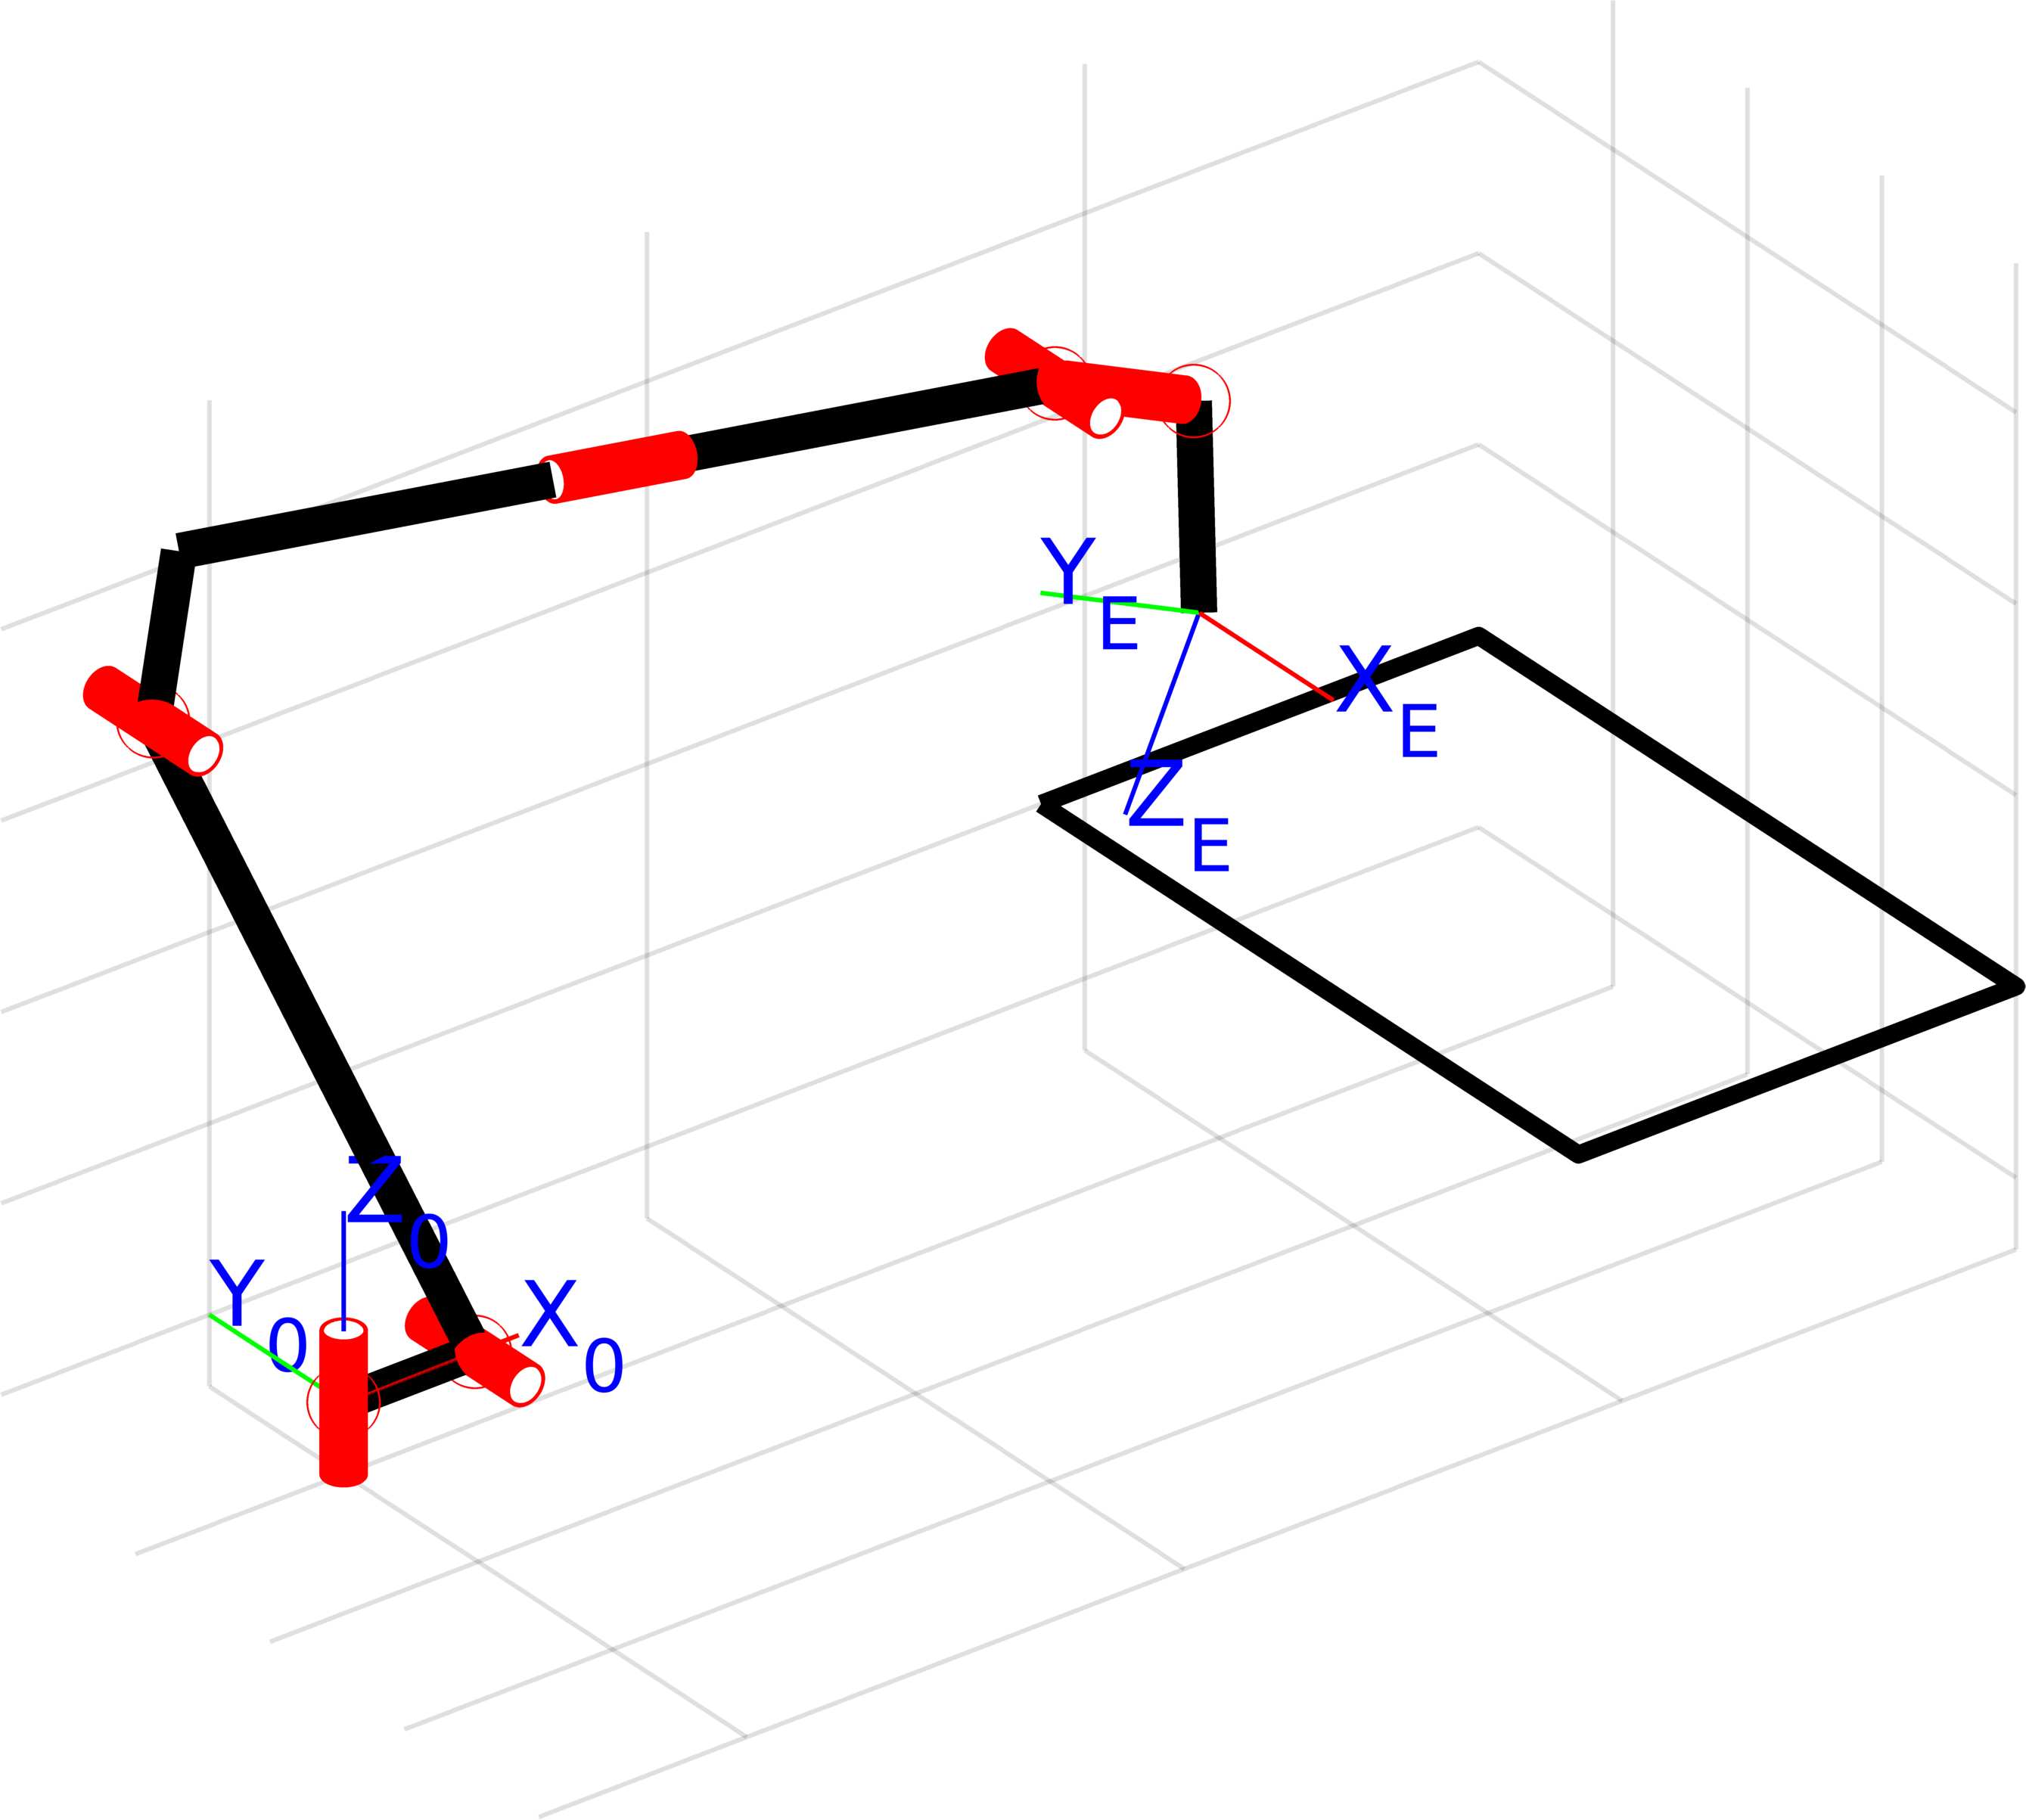
\includegraphics[trim=30 30 0 30, clip, scale=0.7]{serrob_traj_zero_pose.png} % left bottom right top
    \end{minipage}
\end{tabular}
\caption{Left: Table with the kinematic parameters of the industrial manipulator Fanuc M-710 iC/50. Right: sketch of the robot scenario.}
\label{tab:mdh_industrialrobot}
\end{figure}

For the application of the algorithm from (\ref{equ:nullspace}), further extensions were performed to address some practical issues.
First, the simple optimization criterion $h_1$ from (\ref{equ:criterion1}) showed the behavior that violations of the limits of one joint were compensated by improvements for other joints, leaving an invalid solution.
Therefore, it was replaced by the $w_i$-weighted hyperbolic joint limit distance
%
\begin{equation}
h_2(\bm{q})
=
\frac{1}{n} \sum_{i=1}^{n}
w_i
\frac{(q_{i,\mathrm{max}}-q_{i,\mathrm{min}})}{8}
\left(
\frac{1}{(q_{i}-q_{i,\mathrm{min}})^2}
+
\frac{1}{(q_{i}-q_{i,\mathrm{max}})^2}
\right)
\label{equ:criterion2}
\end{equation}
%
from \cite{ZhuQuCaoYan2013} with $n=6$ in this case and the corresponding gradient written element-wise as
\begin{equation}
h_{2,\partial q_i}
=
\frac{\partial h_2}{\partial q_i}
=
w_i
\frac{(q_{i,\mathrm{max}}-q_{i,\mathrm{min}})}{8n}
\left(
\frac{-2}{(q_{i}-q_{i,\mathrm{min}})^3}
+
\frac{-2}{(q_{i}-q_{i,\mathrm{max}})^3}
\right)
\label{equ:criterion2_grad}
\end{equation}
%
with weights set to $w_i=1$.
Additional damping coefficients were introduced, replacing (\ref{equ:nullspace}) with
%
\begin{equation}
{\Delta}\bm{q}^k
=
K_\mathrm{Lim}(\bm{q}) K_\mathrm{Rel}(\bm{q}) (K_\mathrm{T} {\Delta}\bm{q}_{\mathrm{T}}^k + K_\mathrm{N} {\Delta}\bm{q}_{\mathrm{N}}^k),
\label{equ:IK_damping}
\end{equation}
%
where constant damping coefficients $K_\mathrm{T}=0.7$ for ${\Delta}\bm{q}_{\mathrm{T}}^k$ and $K_\mathrm{N}=0.002$ for ${\Delta}\bm{q}_{\mathrm{N}}^k$ were introduced to avoid overshooting of the solution for the prize of slower convergence.
Further damping was introduced for the 3T2R case with optimization\footnote{The 3T3R case and the 3T2R case without optimization do not benefit from this damping term, since the direction of the gradient descent over the limits is unchanged without nullspace.} to reduce a ${\Delta}\bm{q}^{k}$ that would lead to overshoot over the joint limits with $K_\mathrm{Lim}(\bm{q})$, since the new criterion $h_2$ from (\ref{equ:criterion2}) is only meaningfully defined within the joint limits for $q_{i,\mathrm{min}} < q_i < q_{i,\mathrm{max}}$.
The value $K_\mathrm{Lim}=1$ is set if no limits would be violated by the increment ${\Delta}\bm{q}^k$.
The maximum step size for one iteration $\Delta\bm{q}$ was ensured with $K_\mathrm{Rel}(\bm{q})$ to stay below 5\,\% of the joint limit range to prevent leaving the validity of the first-order linearization of (\ref{equ:taylor_phi}). For lower increments, $K_\mathrm{Rel}=1$ holds.
The damping terms are always applied to the full vector and not to single elements and therefore only change the norm and not the direction of ${\Delta}\bm{q}^k$.

The results of the inverse kinematics for different settings are given in Fig.\,\ref{fig:serrob_traj_3T2R}, where the representative joint coordinates $q_1$, $q_2$ and $q_5$ as well as the optimization criterion (\ref{equ:criterion2}) are depicted for the trajectory from Fig.\,\ref{tab:mdh_industrialrobot}.
The positions are normalized to the joint limits from -1 to 1.
The first three lines represent IKP solutions with a given constant end-effector orientation of $-150^\circ$, $-15^\circ$ and $45^\circ$ and the 3T3R algorithm.
The 3T2R algorithm without nullspace optimization is plotted with dotted lines for the same starting configurations as the 3T3R case with the same colors.
The 3T2R case with optimization is plotted as the green line with triangle markers.
%
\begin{figure}[tb]
	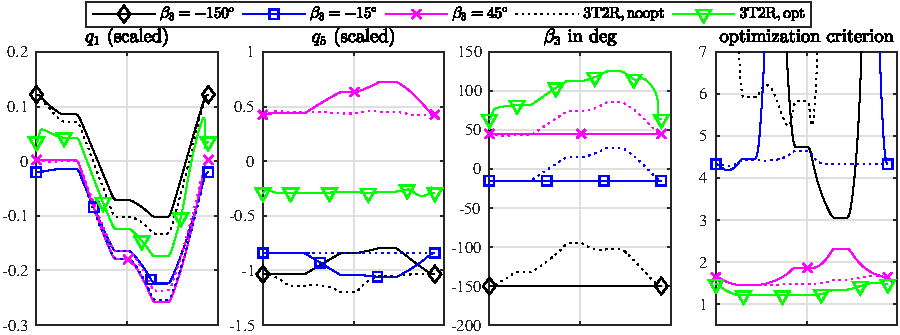
\includegraphics{serrob_traj_nullspace_optim.pdf}
	\caption{Results of the inverse kinematics with different settings for the trajectory of Fig.\,\ref{tab:mdh_industrialrobot}.}
	\label{fig:serrob_traj_3T2R}
\end{figure} 
%
It can be observed, that the optimization of the criterion leads to the best solution of the IKP.
The 3T3R solution with $\beta_3=-150^\circ$ has a lower (i.\,e. better) value for $h_2$, but this represents an invalid solution, as can be seen for the values for $q_5$, where the black line exceeds the upper limit and leaves the domain of the criterion.
The line for the criterion for $\beta_3=-15^\circ$ exceeds the limits of the plot.
This exposes the need for keeping the solution always within the limits by the measures described.
The 3T2R IK without optimization tends to lower changes in the joint positions than the 3T3R IK, since this corresponds to the solution of the matrix pseudo-inverse in (\ref{equ:nullspace}).


\subsection{Statistic Results for the Inverse Kinematics of Serial Link Chains}
\label{sec:Ergebnisse_IK_Statistik}

To emphasize the generality of the presented approach, the inverse kinematics is solved for a set of 309 serial kinematic chains with six joints.
This set of six-DoF kinematics is generated by permutations of their Denavit-Hartenberg parameters and is reduced with the isomorphism detection of \cite{RamirezKotOrt2015} to a minimal set, representing all possible six-DoF serial kinematics with full mobility.
The approach is similar to the results of the evolutionary morphology of parallel robot leg chains of \cite{Gogu2008}.
In contrast to the trajectory evaluation in the previous section focusing on nullspace optimization, the inverse kinematics is solved in this section for arbitrary reachable poses of the serial chain in its workspace.
The poses are generated by the forward kinematics of 50 different joint configurations of the chains uniformly distributed between the joint limits of $\pm \pi$ for rotational joints and $\pm0.5\,\mathrm{m}$ for prismatic joints.
Additionally, the Denavit Hartenberg parameters were set to 50 different sets of uniformly distributed parameters between $0$ and $1$ meters or radians resulting to 2500 combinations for each of the 309 robots in total.
The inital value $\bm{q}^0$ for the solution of the IKP of (\ref{equ:IKP_maintask}) and
(\ref{equ:nullspace}) was set to random values from a uniform distribution within the joint limits.
The following modifications were performed additionally to the ones described in the previous section to increase the efficiency of the algorithm for solving without the good initial values of the trajectory case.
The combined optimization criterion
%
\begin{equation}
h_3(\bm{q})
=
K_{h1} h_1(\bm{q}) + K_{h2} h_2(\bm{q})
\label{equ:criterion3}
\end{equation}
%
was used with empirically determined values of $K_{h1}=0.99$ and $K_{h2}=0.01$ in (\ref{equ:criterion3}) and damping coefficients $K_{\mathrm{T}}=0.6$ and $K_{\mathrm{N}}=0.01$.
The weights $w_i$ of (\ref{equ:criterion2}) were set to 0 in case of joint limit violations for joint $i$, therefore using $h_2$ only for joints within their limits.
The damping term for limit violation was not used in this evaluation, resulting to $K_\mathrm{Lim}(\bm{q})=1$, since for initial values far away from the solution, intermediate steps with limit violations may be required.
%The settings were chosen to allow temporary violations of the joint limits during the convergence to the IK solution.
Using only $h_1$ for joints out of their limits draws their positions $q_i$ back into the allowed region.
The term $h_2$ prevents the algorithm from approaching the limits.
%
A maximum of 15 tries with random initial values was allowed to search for a solution of the IKP within the limits.
After that, five more tries were allowed to find a solution violating the limits, but presenting a solution of the IKP to be able to distinguish the two cases.
A success of the IK is defined as a solution within the joint limits.

The aggregated results are presented as histograms in Fig.\,\ref{fig:serrob_ik_hist_cdf} for different settings of the algorithm.
The histograms show, that for the worst case in 3T2R (3T3R) tasks, the success rate is 87\,\% (69\,\%), marked by the position of the first bars in Fig.\,\ref{fig:serrob_ik_hist_cdf}\,(a) and (c).
These results can be vastly improved by setting the initial guess $\bm{q}^0$ within 20\,\% around the pose, from which the desired end-effector pose has been calculated.
This improves the worst success rate of all robots to 98\,\% for 3T2R (Fig.\,\ref{fig:serrob_ik_hist_cdf}\,b) and 95\,\% for 3T3R tasks (Fig.\,\ref{fig:serrob_ik_hist_cdf}\,d).


%
\begin{figure}[tb]
    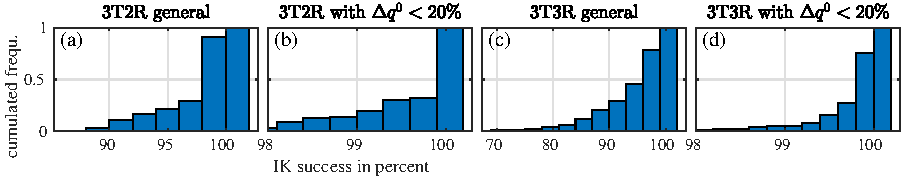
\includegraphics{serrob_ik_hist_cdf_all.pdf}
    \caption{Histograms with cumulated frequency of the IK success for all robots with different settings: 3T2R tasks (a-b) vs. 3T3R tasks (c-d) and arbitrary initial value (a,c) vs. initial value near goal position.}
    \label{fig:serrob_ik_hist_cdf}
\end{figure} 
%

A detailed investigation on the success rates of all serial chains is performed in Fig.\,\ref{fig:serrob_ik_hist}.
The 309 robot kinematics are sorted according to their number of rotational joints and are listed on the horizontal axis of the figure: They contain three rotational joints up to no.\,98, four R-joints up to no.\,240, and five R-joints up to no.\,301.
The first 240 kinematic chains with more than one prismatic joint can be seen as a rather academic example and are listed for the sake of completeness.
The most prominent chains are the UPS-chain from Sec.\,\ref{sec:Ergebnisse_IK_Parallel} at no.\,266 and the six-DoF industrial robot from Sec.\,\ref{sec:Ergebnisse_Seriell} at no.\,309.
%The general kinematics of the industrial robot has 14 instead of the six kinematics parameters in Fig.\,\ref{tab:mdh_industrialrobot}.
Each bar represents the relative frequency of the IK result state in percent for one robot. 
Beginning at the bottom, the number of tries necessary for the solution of the IKP is marked with colors from bright green to orange.
Only cases with a violation of the limits (bright red) or wrong position (dark red) correspond to a failure of the algorithm highlighted in the analysis of Fig.\,\ref{fig:serrob_ik_hist_cdf}.
% The general kinematics 266 can be transformed into the UPS chain by setting all of the 14 parameters to specific values.
The subfigures (a)-(d) of Fig.\,\ref{fig:serrob_ik_hist} correspond to the ones in Fig.\,\ref{fig:serrob_ik_hist_cdf}.
It can be observed, that the quality of the results is clustered according to the kinematic groups.
Structures with at most one P-joint show a considerably better performance of the algorithm with a worst success rate of 97.16\,\% for five R-joints %(at no.\,xx) 
and 99.36\,\% for six R-joints %(at no.\,306) 
for the 3T2R case (a).


\begin{figure}[tb]
    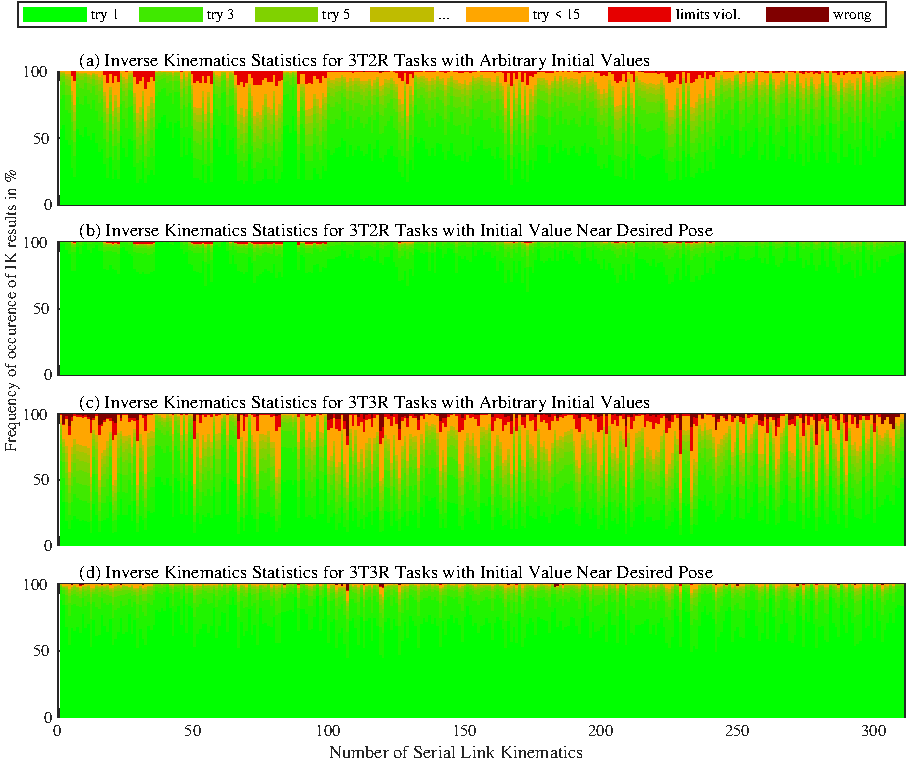
\includegraphics{serrob_ik_hist_all.pdf}
    \caption{Detailed Statistics of the success of the inverse kinematics algorithm for 3T2R tasks (a-b) and 3T3R tasks (c-d). The Success of the IK solver is shown in different shades of green for increasing numbers of required tries. Different initial values $\bm{q}^0$ are distinguished in (a,c) and (b,d).}
    \label{fig:serrob_ik_hist}
\end{figure} 



\subsection{Resolution of Functional Redundancy of a Parallel Robot in 3T2R tasks}
\label{sec:Ergebnisse_IK_Parallel}

%\color{gray}
%\begin{itemize}
%    \item Beispiel IK-Optimierung über Trajektorie (Parameter ähnlich wählen wie in \cite{MerletPerDan2000}).
%\end{itemize}
%\color{black}

As elaborated in Sec.\,\ref{sec:ZB_PKM} and \ref{sec:ZB_Anwendung}, the solution of the IKP for 3T2R and 3T3R tasks is necessary to solve the problem for parallel robots.
Therefore the evaluation for parallel robots in this section is preceded by the examples for serial link chains in the previous sections.
The basic concept is shown for parallel robots at the example of the 6UPS structure following a trajectory.
This robot belongs to the first class presented in Sec.\,\ref{sec:parrob_classification}, which is primarily addressed in this paper.

%\begin{figure}[tb]
%	\begin{tabular}[t]{l r}
%		$\bm{x}_\mathrm{t}^0=\begin{bmatrix}0&0&0.5\,m\end{bmatrix}^\transp$
%		\begin{minipage}[t]{7.5cm}
%			\vspace{0.001cm} % wird für bounding box des Bilds benötigt
%			\hspace{1cm}
%			\includegraphics[trim=50 50 50 50, clip, scale=0.7]{parrob_traj_zero_pose.png} % left bottom right top
%		\end{minipage}
%	\end{tabular}
%	\caption{Left: Kinematic parameters of the 6UPS robot. Right: sketch of the robot scenario.}
%	\label{tab:data_hexapod}
%\end{figure}

The robot has a 6-6 structure with symmetric alignment of the universal joint base couplings on a circle with radius $\lVert\bm{r}_{0A_i}\rVert=1\,\mathrm{m}$ and the spherical joint platform couplings on a circle with radius $\lVert\bm{r}_{B_iE}\rVert=0.4\,\mathrm{m}$.
The initial pose was set to $\bm{x}_\mathrm{t}^\transp=[0,0,0.5\,\mathrm{m}]$ and the initial orientation $\bm{x}_\mathrm{r}$ was set to zero, meaning an alignment of base and platform frame.
The joint positions for each leg were defined to have the initial values $\bm{q}_i^\transp=[30^\circ,-30^\circ,0.583\,\mathrm{m},0^\circ,30^\circ,60^\circ]$ for the given initial platform pose to avoid switching $\pm\pi$ within the trajectory and to avoid gimbal-lock-singularities.
The joint limits were set around the resulting zero position to $\pm0.5\,\mathrm{m}$ for the prismatic joint and $\pm60^\circ$ for all single revolute joints representing the universal and spherical joints.
The values are higher than typical values for real robots to emphasize the effect of the nullspace movement in a bigger workspace of the robot.
The settings for the IK solver are similar as in Sec.\,\ref{sec:Ergebnisse_Seriell}, since both case regard solving the IKP for a trajectory.
By further manual tuning, the values $K_\mathrm{N}=0.7$ and $K_\mathrm{Rel}=1$ limiting to 25\,\% of the joint limit range were identified for a good solution of the IKP.

The time evolution of platform pose and optimization criteria is depicted in Fig.\,\ref{fig:parrob_traj_3T2R}.
The reference trajectory can be seen at the platform position in Fig.\,\ref{fig:parrob_traj_3T2R}\,a and the platform orientation expressed in $X$-$Y$-$Z$-Euler angles ($\beta_1$-$\beta_3$) relative to the base frame in Fig.\,\ref{fig:parrob_traj_3T2R}\,b.
The IKP is solved using two different methods: Only solving the IKP for the legs separately, called ``ser. IK'' and ``IK\,1'' in Fig.\,\ref{fig:parrob_traj_3T2R} and solving the IKP for all legs together, called ``par. IK'' and ``IK\,2'' in Fig.\,\ref{fig:parrob_traj_3T2R}.
Both methods perform an optimization with $h_2$ of (\ref{equ:criterion2}).
The first approach only performs this optimization according to Sec.\,\ref{sec:REW_seriell} for the first leg using the 3T2R method and then solves the IKP for all other legs with the 3T3R method.
The second approach uses the optimization for all legs together according to the 3T2R method from Sec.\,\ref{sec:ZB_PKM}.
This results in improved values for the performance criteria depicted in Fig.\,\ref{fig:parrob_traj_3T2R}\,c and Fig.\,\ref{fig:parrob_traj_3T2R}\,d.
Since the first approach does not regard the limits of the following legs, the optimization criterion gives high values indicating many joint limit violations.
The second approach only shows peaks at $t=1.5\,\mathrm{s}$ in Fig.\,\ref{fig:parrob_traj_3T2R}\,d that result from a joint position getting near to the limit, but not exceeding it.

%
\begin{figure}[tb]
	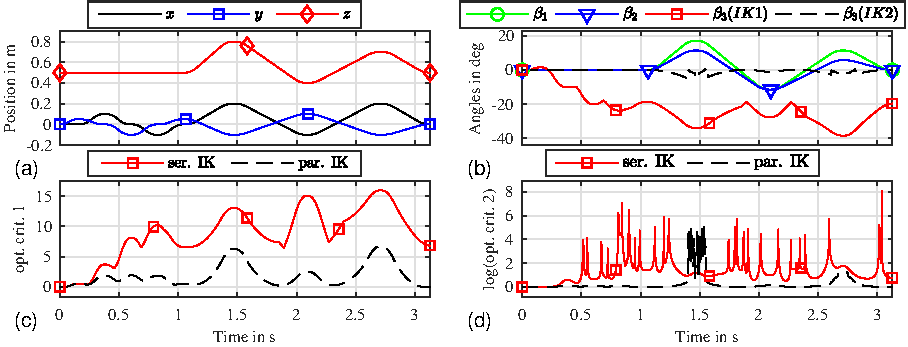
\includegraphics{parrob_traj_results1.pdf}
	\caption{Results of the inverse kinematics of a 6UPS robot in a 3T2R task. (a) platform positions, (b) platform orientation in Euler angles, (c) optimization criterion $h_1(\bm{{q}})$, (d) optimization criterion $h_2(\bm{{q}})$.}
	\label{fig:parrob_traj_3T2R}
\end{figure} 

%\subsection{Determination of the Mobility of a Parallel Robot}
%
%\label{sec:Ergebnisse_Mobilitaet_Delta}
%
%\color{gray}
%\begin{itemize}
%    \item Beispielrechnung Delta-Roboter: Jacobi-Matrix Rang und Null-Einträge
%\end{itemize}
%\color{black}

%%%%%%%%%%%%%%%%%%%%%%%%%%%%%%%%%%%%%%%%%%
\section{Discussion}

%Authors should discuss the results and how they can be interpreted in perspective of previous studies and of the working hypotheses. The findings and their implications should be discussed in the broadest context possible. Future research directions may also be highlighted.

A general kinematics model for parallel robots is introduced to solve the inverse kinematics problem for any kind of parallel robot in tasks with one redundant rotational DoF (3T2R).
The prize of the generality of the approach is the increased size of the geometric matrices, which is $10 \times 11$ for robots with a simple structure instead of $6\times6$ for the non-redundant kinematics and grow up to $35 \times 36$ for general task redundant parallel robots with full mobility.
This makes symbolic calculations of the kinematic matrices impossible, allowing only studies on mobility, singularities and other properties of the Jacobian matrix based on numeric calculations.
The application of the method can therefore be seen mainly in finding optimal trajectories for task redundant parallel robots in milling or drilling scenarios regarding stiffness, dexterity or joint limits.
%This allows to exploit the performance of the mechanisms to full extend.
%
%The complete formulation on the other hand allows a gradient-based analysis of the joint limits of active and passive joints.
%It is 
%The method can be applied to find optimal trajectories for task redundant parallel robots in milling or drilling scenarios regarding stiffness, dexterity or joint limits.
%This allows to exploit the performance of the mechanisms to full extend.
Due to the performance of the method demonstrated at exemplary cases, an online implementation is possible but has to be proved in future works to converge in real-time conditions for specific machines.
The generality of the approach allows to use it in a combined structural and dimensional synthesis sketched in Fig.\,\ref{fig:structdimsynth}, extending the purely structural synthesis of parallel robot kinematics from \cite{Gogu2008,KongGos2005} to a dimensional synthesis of all structures as shown in \cite{RamirezKotOrt2015} for serial robots.

%%%%%%%%%%%%%%%%%%%%%%%%%%%%%%%%%%%%%%%%%%%
%\section{Materials and Methods}
%
%Materials and Methods should be described with sufficient details to allow others to replicate and build on published results. Please note that publication of your manuscript implicates that you must make all materials, data, computer code, and protocols associated with the publication available to readers. Please disclose at the submission stage any restrictions on the availability of materials or information. New methods and protocols should be described in detail while well-established methods can be briefly described and appropriately cited.
%
%Research manuscripts reporting large datasets that are deposited in a publicly available database should specify where the data have been deposited and provide the relevant accession numbers. If the accession numbers have not yet been obtained at the time of submission, please state that they will be provided during review. They must be provided prior to publication.
%
%Interventionary studies involving animals or humans, and other studies require ethical approval must list the authority that provided approval and the corresponding ethical approval code. 

%%%%%%%%%%%%%%%%%%%%%%%%%%%%%%%%%%%%%%%%%%%
%\section{Conclusions}
%
%This section is not mandatory, but can be added to the manuscript if the discussion is unusually long or complex.


%%%%%%%%%%%%%%%%%%%%%%%%%%%%%%%%%%%%%%%%%%
\vspace{6pt} 

%%%%%%%%%%%%%%%%%%%%%%%%%%%%%%%%%%%%%%%%%%
%% optional
%\supplementary{The following are available online at \linksupplementary{s1}, Figure S1: title, Table S1: title, Video S1: title.}

% Only for the journal Methods and Protocols:
% If you wish to submit a video article, please do so with any other supplementary material.
% \supplementary{The following are available at \linksupplementary{s1}, Figure S1: title, Table S1: title, Video S1: title. A supporting video article is available at doi: link.}

%%%%%%%%%%%%%%%%%%%%%%%%%%%%%%%%%%%%%%%%%%
\authorcontributions{conceptualization, M.S. and S.T.; methodology, M.S.; software, M.S.; validation, M.S.; formal analysis, M.S.; writing--original draft preparation, M.S.; writing--review and editing, M.S., S.T., T.O.; supervision, S.T. and T.O.; project administration, T.O.; funding acquisition, S.T. and T.O.}
% , please turn to the  \href{http://img.mdpi.org/data/contributor-role-instruction.pdf}{CRediT taxonomy} for the term explanation. Authorship must be limited to those who have contributed substantially to the work reported.

%%%%%%%%%%%%%%%%%%%%%%%%%%%%%%%%%%%%%%%%%%
\funding{The financial support from the Deutsche Forschungsgemeinschaft (German Research Foundation, DFG) under grant number OR 196/33-1 is gracefully acknowledged.}

%%%%%%%%%%%%%%%%%%%%%%%%%%%%%%%%%%%%%%%%%%
%\acknowledgments{In this section you can acknowledge any support given which is not covered by the author contribution or funding sections. This may include administrative and technical support, or donations in kind (e.g., materials used for experiments).}

%%%%%%%%%%%%%%%%%%%%%%%%%%%%%%%%%%%%%%%%%%
\conflictsofinterest{The authors declare no conflict of interest.} 

%%%%%%%%%%%%%%%%%%%%%%%%%%%%%%%%%%%%%%%%%%
%% optional
\abbreviations{The following abbreviations are used in this manuscript:\\

\noindent 
\begin{tabular}{@{}ll}
PKM & parallel kinematic machine (parallel robot) \\
IKP & inverse kinematics problem \\
DoF & degrees of freedom \\
$x$T$y$R & $x$ translational and $y$ rotational degrees of freedom
\end{tabular}}

%%%%%%%%%%%%%%%%%%%%%%%%%%%%%%%%%%%%%%%%%%
%% optional
\appendixtitles{no} %Leave argument "no" if all appendix headings stay EMPTY (then no dot is printed after "Appendix A"). If the appendix sections contain a heading then change the argument to "yes".
\appendix
\section{Mathematical Symbols for Reciprocal Euler Angles in Inverse Kinematics}
\label{sec:appendix_proof_REW}
%\unskip
%\subsection{}

%\color{gray}
%\begin{itemize}
%	\item Details zu den Partiellen Ableitungen in den verschiedenen Gleichungen
%	\item Genauer Inhalt der Spalten-Operatoren und der Euler-Winkel-Ableitungen
%	\item Herleitung für Zusammenhang Rotationsmatrix-Winkelgeschwindigkeit (Gradienten)
%\end{itemize}
%\color{black}

The following appendix contains additional detailed information about the kinematic constraint formulation of this paper.
Sec.\,\ref{sec:appendix_eulerreciproc} contains a mathematical proof for the properties of reciprocal Euler angles in inverse kinematics, which is only outlined in equ.\,18 of \cite{1_SchapplerTapOrt2019}.
The justification for using the approach of partial derivatives instead of the geometric Jacobian is derived in Sec.\,\ref{sec:appendix_gradient_geomjacobian}.
The matrix operations for the partial derivatives are replicated from \cite{1_SchapplerTapOrt2019} in Sec.\,\ref{sec:appendix_gradient_matrix} and the contents of the single partial derivatives are given in Sec.\,\ref{sec:appendix_content_derivatives} to facilitate the understanding and implementation by the reader.

\subsection{Proof for the Properties of Reciprocal Euler angles}
\label{sec:appendix_eulerreciproc}


This section derives the effect of the reciprocity of Euler-angles at the example of the kinematics description of Sec.\,\ref{sec:REW_seriell} and the frames of Fig.\,\ref{fig:frames_5dof_6dof}\,(b):
%
An end-effector orientation $\bm{\beta}=\bm{x}_{\mathrm{r}}$ gives the rotation matrix\footnote{The matrix rotates vectors from $\ks{E}$ to $\ks{D}$}
%
\begin{equation}
\rotmat{D}{E}(\bm{\beta},\bm{q})
= 
\rotmat{0}{D}^\transp (\bm{\beta})\rotmat{0}{E}(\bm{q})
\label{equ:orierr_1_rotmat}
\end{equation}
%
from the actual end-effector frame $\ks{E}$ to the desired or platform end-effector frame $\ks{D}$,
where using the $X$-$Y$-$Z$-Euler angles and exploiting the properties of $\mathrm{SO(3)}$ rotation matrices yields
%
\begin{equation}
\rotmat{0}{D}^\transp(\bm{\beta})
=
\bm{R}_z(-\beta_3) \bm{R}_y(-\beta_2) \bm{R}_x(-\beta_1)
\end{equation}
%
as introduced in (\ref{equ:def_rmat_xyz}).
With an additional rotation $-\delta$ around the $z$-axis for the desired orientation, the resulting new Euler angles $\bm{\beta}'$ are
%
\begin{equation}
\beta_1'=\beta_1,  \quad \beta_2'=\beta_2,  \quad \beta_3'=\beta_3-\delta.
\end{equation}
%
The additional rotation corresponds to the tool axis defined in Sec.\,\ref{sec:REW_seriell} % and does not influence 3T2R tasks.
and leads to a new residual orientation error expressed as a rotation matrix
%
\begin{align}
    \rotmat{D}{E}(\bm{\beta}',\bm{q})
    &=
    \rotmat{0}{D}^\transp (\bm{\beta}') \rotmat{0}{E}(\bm{q}) \nonumber\\
    &=
    \left(\rotmat{0}{D}(\bm{\beta})\bm{R}_z(-\delta)\right)^\transp \rotmat{0}{E}(\bm{q}) \nonumber \\
    &=
    \bm{R}_z(\delta) \rotmat{0}{D}^\transp (\bm{\beta}) \rotmat{0}{E}(\bm{q}) \nonumber \\
    &=
    \bm{R}_z(\delta) \rotmat{D}{E}(\bm{\beta},\bm{q}).
    \label{equ:orierr_2_rotmat}
\end{align}
%
The first residual orientation error from (\ref{equ:orierr_1_rotmat}) corresponding to $\bm{\beta}$ is defined as a rotation matrix
%
% Quelle: equations/R1.txt (aus ikfr_paper_equations.mw)
\begin{align}
    \rotmat{D}{E}(\bm{\beta},\bm{q})
    =
    \begin{bmatrix}
        {n_x}&{o_x}&{a_x} \\
        {n_y}&{o_y}&{a_y} \\ 
        {n_z}&{o_z}&{a_z} \\ 
    \end{bmatrix}
    \label{equ:orierr_1_rotmat_def}
\end{align}
%
and as a $Z$-$Y$-$X$-Euler angle representation\footnote{Utilizing the sign-aware operator $\arctantwo(y,x)$ instead of $\arctan(y/x)$ allows angles to be in $(-\pi,+\pi]$, removes ambiguities and provides global differentiability.}
%
% Quelle: equations/alpha1.txt (aus ikfr_paper_equations.mw)
\begin{align}
    \bm{\alpha}
	=
	\begin{bmatrix}
	\alpha_1 \\
	\alpha_2 \\
	\alpha_3
    \end{bmatrix}
	=
    \begin{bmatrix}
        \arctantwo \left( {n_y} , { n_x} \right) \\ 
        \arctantwo \left( -{n_z} , \sqrt {{{a_z}}^{2}+{{ o_z}}^{2}} \right) \\ 
        \arctantwo \left( {o_z} , {a_z} \right)
    \end{bmatrix}.
    \label{equ:alpha_zyx}
\end{align}
%
The second residual corresponding to $\bm{\beta}'$ only differs regarding the additional rotation $\delta$. Combining (\ref{equ:orierr_2_rotmat}) and (\ref{equ:orierr_1_rotmat_def}) leads to
%
% Quelle: equations/R2.txt (aus ikfr_paper_equations.mw)
\begin{align}
    \rotmat{D}{E}(\bm{\beta}',\bm{q})
    =
    \begin{bmatrix}
    {n'_x}&{o'_x}&{a'_x} \\
    {n'_y}&{o'_y}&{a'_y} \\ 
    {n'_z}&{o'_z}&{a'_z} \\ 
    \end{bmatrix}
    = 
    \left[ \begin {array}{ccc} { C_{\delta}}\,{n_x}-{ S_{\delta}}\,{ n_y}&{ C_{\delta}}\,{o_x}-{ S_{\delta}}\,{o_y}&{ C_{\delta}}\,{ a_x}-{ S_{\delta}}\,{a_y}\\ \noalign{\medskip}{ C_{\delta}}\,{n_y}+ { S_{\delta}}\,{n_x}&{ C_{\delta}}\,{o_y}+{ S_{\delta}}\,{o_x}&{  C_{\delta}}\,{a_y}+{ S_{\delta}}\,{a_x}\\ \noalign{\medskip}{ n_z}&{o_z}&{a_z}\end {array} \right], \nonumber
\end{align}
%
where $C_{\delta}=\mathrm{cos}(\delta)$ and $S_{\delta}=\mathrm{sin}(\delta)$.
The $Z$-$Y$-$X$-Euler angles from this rotation matrix are
%
% Quelle: equations/alpha2.txt (aus ikfr_paper_equations.mw)
\begin{equation}
\bm{\alpha}'
=
\begin{bmatrix}
\alpha_1' \\
\alpha_2' \\
\alpha_3'
\end{bmatrix}
=
\begin{bmatrix}
\arctantwo \left( {n'_y} , { n'_x} \right) \\ 
\arctantwo \left( -{n'_z} , \sqrt {{{a'_z}}^{2}+{{ o'_z}}^{2}} \right) \\ 
\arctantwo \left( {o'_z} , {a'_z} \right)
\end{bmatrix}
=
\begin{bmatrix}
\arctantwo \left( ({  C_{\delta}}\,{n_y}+{ S_{\delta}}\,{n_x}) , ({ C_{\delta}}\,{n_x}-{  S_{\delta}}\,{n_y}) \right) \\
\arctantwo \left( -{n_z} , \sqrt {{{a_z}}^{2}+{{ o_z}}^{2}} \right) \\
\arctantwo \left( {o_z} , {a_z} \right)
\end{bmatrix},
\end{equation}
%
where $\delta$  only influences the first component $\alpha_1'$.
This allows the conclusion, that $\beta_3$ only influences $\alpha_1$ and results in the dependencies
%
\begin{align}
    \alpha_1'&=\alpha_1'(\bm{q},\beta_1,\beta_2,\beta_3)\\
    \alpha_2'&=\alpha_2'(\bm{q},\beta_1,\beta_2) =\alpha_2\\
    \alpha_3'&=\alpha_3'(\bm{q},\beta_1,\beta_2) =\alpha_3
\end{align}
%
with the consequences for the kinematic modeling of robots in 3T2R tasks described in Sec.\,\ref{sec:REW_seriell}.

\subsection{Relation of the Gradient Matrices to the Geometric Jacobian of the Serial Chain}
\label{sec:appendix_gradient_geomjacobian}

%\color{gray}
%\begin{itemize}
%	\item Methode mit Orientierungs-Residuum basierend auf Euler-Winkeln wurde in \cite{GoldenbergBenFen1985} eingeführt. Dort wurde der Gradient mit der geometrischen Jacobi-Matrix erklärt, ohne genauere Rechnung.
%	\item Mathematischer Beweis hier, dass das nicht möglich ist, da sich der Gradient auf den Orientierungsfehler bezieht und die Jacobi auf die absolute Orientierung
%	\item Nur für den Fall, dass die ZB=0 sind, sind die Darstellungen überführbar.
%\end{itemize}
%\color{black}

As introduced in Sec.\,\ref{sec:ZB_Anwendung}, the rotational part of the gradient matrices can not be derived with the commonly available Jacobian of the serial link kinematics of the legs.
Defining the residual of the orientation for the inverse kinematics with Euler angles was first introduced in \cite{GoldenbergBenFen1985}, where the calculation of the partial derivatives was referred to the geometric Jacobian without further clarification.
The relationship between the gradient matrices from Sec.\,\ref{sec:ZB_Anwendung} and the Jacobian can be obtained by comparing the platform or end-effector velocity 
%
\begin{equation}
\dot{\bm{x}} = \bm{J}_1 \dot{\bm{q}}_1,
\quad
\begin{bmatrix}
\dot{\bm{x}}_\mathrm{t}\\
\dot{\bm{x}}_\mathrm{r}
\end{bmatrix}
 = 
\begin{bmatrix}
 \bm{J}_{\mathrm{t},1}(\bm{q}_1)\\
 \bm{J}_{\mathrm{r},1}(\bm{q}_1) 
\end{bmatrix}
\dot{\bm{q}}_1
\label{equ:diffkin1_jacobi}
\end{equation}
%
obtained with the Jacobian with the velocity obtained by the gradient matrices of (\ref{equ:Phi_def}).
Using the differential form (\ref{equ:constr_diff}) only for the first kinematic leg chain of the parallel robot gives
%
\begin{equation}
\frac{\mathrm{d}}{\mathrm{d}t} \bm{\Phi}_1(\bm{q}_1,\bm{x})
=
\bm{\Phi}_{1,\bm{q}}(\bm{q}_1,\bm{x}) \dot{\bm{q}}_1 + \bm{\Phi}_{1,\bm{x}}(\bm{q}_1,\bm{x}) \dot{\bm{x}} 
=
\bm{0}
\label{equ:constr_diff1}
\end{equation}
%
and results reorganized to the form of (\ref{equ:diffkin1_jacobi}) with (\ref{equ:Phi_1_grad_q}) and (\ref{equ:Phi_1_grad_x}) to
%
\begin{equation}
\begin{bmatrix}
\dot{\bm{x}}_\mathrm{t}\\
\dot{\bm{x}}_\mathrm{r}
\end{bmatrix}
=
-
\begin{bmatrix}
-\bm{1} & \bm{0} \\
\bm{0} & \bm{\Phi}_{\mathrm{r},1,\partial\bm{x}_\mathrm{r}}^{-1}
\end{bmatrix}
\begin{bmatrix}
\bm{\Phi}_{\mathrm{t},1,\partial\bm{q}_1}
&
\bm{\Phi}_{\mathrm{r},1,\partial\bm{q}_1}
\end{bmatrix}
\dot{\bm{q}}_1
=
\begin{bmatrix}
\bm{\Phi}_{\mathrm{t},1,\partial\bm{q}_1} & \bm{0} \\
\bm{0} & -\bm{\Phi}_{\mathrm{r},1,\partial\bm{x}_\mathrm{r}}^{-1} \bm{\Phi}_{\mathrm{r},1,\partial\bm{q}_1}
\end{bmatrix}
\dot{\bm{q}}_1.
\label{equ:diffkin1_gradmat}
\end{equation}
%
By equating coefficients of (\ref{equ:diffkin1_jacobi}) and (\ref{equ:diffkin1_gradmat}) the relations
%
\begin{align}
\bm{\Phi}_{1,\bm{q}}(\bm{q}_1)
&=
-\bm{\Phi}_{1,\bm{x}}(\bm{q}_1,\bm{x})
\bm{J}_1(\bm{q}_1),
\label{equ:KoeffVgl_Phi1d1}
\\
\bm{\Phi}_{\mathrm{t},1,\partial\bm{q}_1}(\bm{q}_1)
&=
\bm{J}_{\mathrm{t},1}(\bm{q}_1)\quad\mathrm{and}
\label{equ:KoeffVgl_Phi1td1}
\\
\bm{\Phi}_{\mathrm{r},1,\partial\bm{q}_1}(\bm{q}_1,\bm{x})
&=
-\bm{\Phi}_{\mathrm{r},1,\partial\bm{x}_\mathrm{r}}(\bm{q}_1,\bm{x}) \bm{J}_{\mathrm{r},1}(\bm{q}_1)
\label{equ:KoeffVgl_Phi1rd1}
\end{align}
%
can be obtained between the gradient matrices and the analytic Jacobian of the serial leg chain.
The dependency on $\bm{q}_1$ and $\bm{x}$ has been added to highlight the main requirement, namely the zero equality condition of (\ref{equ:constr_diff1}).
In the inverse kinematics procedure of Sec.\,\ref{sec:ZB_Anwendung_IK_grad} the residual at step $k$ in (\ref{equ:taylor_phi}) is unequal to zero.
For the partial derivative (\ref{equ:grad_Phi_1_x})/I a value of $\rotmato{D}{E} \ne \bm{1}$ will be inserted in (\ref{equ:alpha_xyz_diff_R}), which will break (\ref{equ:KoeffVgl_Phi1rd1}).
The translational part is unaffected, as can be seen in (\ref{equ:KoeffVgl_Phi1td1}).
%Since the term $\bm{\Phi}_{\mathrm{r},1,\partial\bm{x}_\mathrm{r}}$ depends on $\bm{q}_1$ \emph{and} $\bm{x}$

\subsection{Matrix Operations for Partial Derivatives}
\label{sec:appendix_gradient_matrix}

To simplify the calculations of the gradient matrices of the residuals in Sec.\,\ref{sec:ZB_Anwendung}, operators for matrices are replaced by operators for vectors, to avoid differentiating matrices or w.r.t. matrices which would require multi-dimensional tensors.
The column operator $\overline{\bm{R}}$ for rotation matrices $\bm{R}$ to stack the coordinate systems unit vectors $\bm{n},\bm{o},\bm{a} \in {\mathbb{R}}^{3}$ vertically instead of horizontally is defined as
%
\begin{equation}
\overline{\bm{R}}(\bm{R})=\begin{bmatrix}
\bm{n} \\ \bm{o} \\ \bm{a}
\end{bmatrix} \in {\mathbb{R}}^{9}
\quad
\mathrm{with}
\quad
\bm{R}=\begin{bmatrix}
\bm{n} & \bm{o} & \bm{a}
\end{bmatrix}
=
\begin{bmatrix}
{n_x}&{o_x}&{a_x} \\
{n_y}&{o_y}&{a_y} \\ 
{n_z}&{o_z}&{a_z} \\ 
\end{bmatrix}
\in \mathrm{SO}(3)
\label{equ:def_rotmat}
\end{equation}
%
to avoid differentiating matrices or w.r.t. matrices.
The special properties of the $\mathrm{SO}(3)$ group are not exploited and the operator can be used for ${\mathbb{R}}^{3\times3}$ as well.
Matrix multiplication is expressed with the matrix product operator $\overline{\Pi}$
%
such that
%
\begin{equation}
\rotmato{1}{3}
=
\overline{\prod}\left( \rotmato{1}{2}, \rotmato{2}{3}\right)
=
\overline{\bm{R}}(\rotmat{1}{3})
\quad
\mathrm{with}
\quad
\rotmat{1}{3}
=
\rotmat{1}{2}
\rotmat{2}{3}.
\label{equ:matprod}
\end{equation}
%
The transposition operator $\bm{P}_\transp$ is a $9 \times 9$ permutation matrix such that
%
\begin{equation}
\rotmato{2}{1}
=
\bm{P}_\transp \rotmato{1}{2}
=
\overline{\bm{R}}(\rotmat{1}{2}^\transp)
=
\rotmato{1}{2}^\transp
\in {\mathbb{R}}^{9}
\enspace
\mathrm{with}
\enspace
\rotmat{2}{1}
=
\rotmat{1}{2}^\transp
\in \mathrm{SO}(3)
\enspace
\mathrm{and}
\enspace
\rotmato{1}{2}=\overline{\bm{R}}(\rotmat{1}{2})
.
\label{equ:transposition_operator}
\end{equation}
%
Writing $\rotmato{1}{2}^\transp$ instead of $\bm{P}_\transp \rotmato{1}{2}$ serves for the clarity of the expressions (\ref{equ:grad_Phi_1_q},\ref{equ:grad_Phi_1_x},\ref{equ:grad_Phi_j_qj},\ref{equ:grad_Phi_j_q1}) and overloads the transposition operator for ${\mathbb{R}}^{9}$ noted with the bar.
%\color{gray}
%The Euler angles can be calculated from the general rotation matrix $\bm{R}$ of (\ref{equ:def_rotmat}) in the same way as before using these operators with the notation
%%
%\begin{equation}
%\bm{\beta}(\overline{\bm{R}})
%=
%\bm{\beta}(\bm{R})
%=
%\begin{bmatrix}
%xxx \arctantwo \left( {n_y} , { n_x} \right) \\ 
%xxx \arctantwo \left( -{n_z} , \sqrt {{{a_z}}^{2}+{{ o_z}}^{2}} \right) \\ 
%xxx \arctantwo \left( {o_z} , {a_z} \right)
%\end{bmatrix}
%\label{equ:beta_def_rotmat_xyz}
%\end{equation}
%%
%at the $X$-$Y$-$Z$ example.
%\color{black}

\subsection{Contents of the Partial Derivatives}
\label{sec:appendix_content_derivatives}

The single expressions derived in Sec.\,\ref{sec:ZB_Anwendung} can be calculated with low computational effort from the definition of the $X$-$Y$-$Z$- and $Z$-$Y$-$X$-Euler angles from (\ref{equ:def_rmat_xyz}), (\ref{equ:def_rmat_zyxr}) and (\ref{equ:alpha_zyx}).
With $\overline{\bm{R}}=[n_x,n_y,n_z ,o_x,o_y,o_z,a_x,a_y,a_z]^\transp$ the gradient ``I'' in (\ref{equ:grad_Phi_1_q},\ref{equ:grad_Phi_1_x},\ref{equ:grad_Phi_j_qj},\ref{equ:grad_Phi_j_q1}) for $Z$-$Y$-$X$ angles becomes
% Quelle: equations/dalphadRb.txt (aus ikfr_pkm_paper_equations.mw; danach equations_postprocess.sh)
%
\begin{equation}
\frac{\partial \bm{\alpha}(\overline{\bm{R}})}{\partial \overline{\bm{R}}}
=
\left[ \begin {array}{ccccccccc} -{\frac {{n_y}}{{{n_x}}^{2}+{{ n_y}}^{2}}}&{\frac {{n_x}}{{{n_x}}^{2}+{{n_y}}^{2}}}&0&0&0 &0&0&0&0\\ \noalign{\medskip}0&0&-\sqrt {{{a_z}}^{2}+{{o_z}}^{2} }&0&0&{\frac {{n_z}\,{o_z}}{\sqrt {{{a_z}}^{2}+{{o_z}}^{2} }}}&0&0&{\frac {{n_z}\,{a_z}}{\sqrt {{{a_z}}^{2}+{{o_z}}^{ 2}}}}\\ \noalign{\medskip}0&0&0&0&0&{\frac {{a_z}}{{{a_z}}^{2}+{ {o_z}}^{2}}}&0&0&-{\frac {{o_z}}{{{a_z}}^{2}+{{o_z}}^{2}}} \end {array} \right] 
\label{equ:alpha_xyz_diff_R}
\end{equation}
%
and the inverse gradient ``IV'' in (\ref{equ:grad_Phi_1_x}) for $X$-$Y$-$Z$ angles yields
%
% Quelle: equations/R2b_dxyz.txt (aus ikfr_paper_equations.mw)
\begin{align}
\frac{\partial \overline{\bm{R}}(\bm{\beta})}{\partial \bm{\beta}}
=
\small
\begin{bmatrix}
    0&-{ S_2}\,{ C_3}&-{ C_2}\,{ S_3}
    \\ { C_1}\,{ S_2}\,{ C_3}-{ S_1}\,{ S_3}&{
        S_1}\,{ C_2}\,{ C_3}&-{ S_1}\,{ S_2}\,{ S_3}+{ C_1}\,{
        C_3}\\ { S_1}\,{ S_2}\,{ C_3}+{ C_1}\,{
        S_3}&-{ C_1}\,{ C_2}\,{ C_3}&{ C_1}\,{ S_2}\,{ S_3}+{
        S_1}\,{ C_3}\\ 0&{ S_2}\,{ S_3}&-{ C_2}\,
    { C_3}\\ -{ C_1}\,{ S_2}\,{ S_3}-{ S_1}\,{
        C_3}&-{ S_1}\,{ C_2}\,{ S_3}&-{ S_1}\,{ S_2}\,{ C_3}-{
        C_1}\,{ S_3}\\ -{ S_1}\,{ S_2}\,{ S_3}+{
        C_1}\,{ C_3}&{ C_1}\,{ C_2}\,{ S_3}&{ C_1}\,{ S_2}\,{
        C_3}-{ S_1}\,{ S_3}\\ 0&{ C_2}&0
    \\ -{ C_1}\,{ C_2}&{ S_1}\,{ S_2}&0
    \\ -{ S_1}\,{ C_2}&-{ C_1}\,{ S_2}&0
    \end {bmatrix}
\label{equ:rotmat_diff_beta}
\end{align}
%
with $C_i=\mathrm{cos}(\beta_i)$, $S_i=\mathrm{sin}(\beta_i)$.
The property
%
\begin{equation}
\left(\frac{\partial \bm{\beta}}{\partial \overline{\bm{R}}}\right)
\left(\frac{\partial \overline{\bm{R}}(\bm{\beta})}{\partial \bm{\beta}}\right)
=
\bm{1} \in {\mathbb{R}}^{3 \times 3}
\end{equation}
%
can be used to test the implementation, if (\ref{equ:alpha_xyz_diff_R}, \ref{equ:rotmat_diff_beta}) are defined for the same Euler-angle notation.
The gradient of the matrix product (\ref{equ:matprod}) w.r.t. the second factor used in (\ref{equ:grad_Phi_1_q})/II, (\ref{equ:grad_Phi_1_x})/III, (\ref{equ:grad_Phi_j_qj})/II and (\ref{equ:grad_Phi_j_q1})/III is
%
\begin{equation}
\frac{\partial }{\partial \overline{\bm{R}}_2}
\overline{\prod}\left( \overline{\bm{R}}_1, \overline{\bm{R}}_2\right)
=
\begin{bmatrix}
\bm{R}_1 & \bm{0} & \bm{0} \\
\bm{0} & \bm{R}_1 & \bm{0} \\
\bm{0} & \bm{0} & \bm{R}_1  \\
\end{bmatrix}
\label{equ:diff_prod_mat2}
\end{equation}
%
and to complete the enumeration the gradient w.r.t. the first factor is
%
\begin{equation}
\frac{\partial }{\partial \overline{\bm{R}}_1}
\overline{\prod}\left( \overline{\bm{R}}_1, \overline{\bm{R}}_2\right)
=
\begin{bmatrix}
{\mathrm{diag}}(n_x)&{\mathrm{diag}}(o_x)&{\mathrm{diag}}(a_x) \\ {\mathrm{diag}}(n_y)&{\mathrm{diag}}(o_y)&{\mathrm{diag}}(a_y)\\ {\mathrm{diag}}(n_z)&{\mathrm{diag}}(o_z)&{\mathrm{diag}}(a_z)
\end{bmatrix},
\label{equ:diff_prod_mat1}
\end{equation}
%
where $n_x,n_y,...$ are the entries of $\bm{R}_2$ and the $\mathrm{diag}$-matrices are $3 \times 3$.
By transposing the elements of the matrix product (\ref{equ:matprod}), only the first form (\ref{equ:diff_prod_mat2}) had to be used in this paper.

%%%%%%%%%%%%%%%%%%%%%%%%%%%%%%%%%%%%%%%%%%
% Citations and References in Supplementary files are permitted provided that they also appear in the reference list here. 

%=====================================
% References, variant A: internal bibliography
%=====================================
\reftitle{References}
%\begin{thebibliography}{999}
%% Reference 1
%\bibitem[Author1(year)]{ref-journal}
%Author1, T. The title of the cited article. {\em Journal Abbreviation} {\bf 2008}, {\em 10}, 142--149.
%% Reference 2
%\bibitem[Author2(year)]{ref-book}
%Author2, L. The title of the cited contribution. In {\em The Book Title}; Editor1, F., Editor2, A., Eds.; Publishing House: City, Country, 2007; pp. 32--58.
%\end{thebibliography}

% The following MDPI journals use author-date citation: Arts, Econometrics, Economies, Genealogy, Humanities, IJFS, JRFM, Laws, Religions, Risks, Social Sciences. For those journals, please follow the formatting guidelines on http://www.mdpi.com/authors/references
% To cite two works by the same author: \citeauthor{ref-journal-1a} (\citeyear{ref-journal-1a}, \citeyear{ref-journal-1b}). This produces: Whittaker (1967, 1975)
% To cite two works by the same author with specific pages: \citeauthor{ref-journal-3a} (\citeyear{ref-journal-3a}, p. 328; \citeyear{ref-journal-3b}, p.475). This produces: Wong (1999, p. 328; 2000, p. 475)

%=====================================
% References, variant B: external bibliography
%=====================================
\externalbibliography{yes}
\bibliography{references}

%%%%%%%%%%%%%%%%%%%%%%%%%%%%%%%%%%%%%%%%%%
%% optional
%\sampleavailability{Samples of the compounds ...... are available from the authors.}

%% for journal Sci
%\reviewreports{\\
%Reviewer 1 comments and authors’ response\\
%Reviewer 2 comments and authors’ response\\
%Reviewer 3 comments and authors’ response
%}

%%%%%%%%%%%%%%%%%%%%%%%%%%%%%%%%%%%%%%%%%%
\end{document}

